\documentclass[a4paper,12pt]{article}
\usepackage[brazil, english]{babel}
\usepackage[utf8]{inputenc}
\usepackage[T1]{fontenc}
\usepackage{geometry}
\usepackage{setspace}
\usepackage{titlesec}
\usepackage{hyperref}
\usepackage{graphicx}
\usepackage{caption}
\usepackage{subcaption}
\usepackage{fancyhdr}
\setlength{\headheight}{15pt}
\addtolength{\topmargin}{-2.5pt}
\usepackage{xcolor}
\usepackage{amsmath, amssymb, bm}
\usepackage{mathtools}
\usepackage{cancel}
\usepackage{tikz}
\usepackage{newunicodechar}
\usepackage{ragged2e}
\usepackage{setspace}
\usepackage{tikz-3dplot} % Necessário para coordenadas 3D
\usetikzlibrary{intersections}
\usepackage{siunitx}
\usetikzlibrary{3d, arrows.meta}
\usepackage{booktabs}


\usepackage{color}
\definecolor{myblue}{rgb}{.8, .8, 1}

\definecolor{ao(english)}{rgb}{0.0, 0.5, 0.0}

\usepackage{amsmath}
\usepackage{empheq}

\newlength\mytemplen
\newsavebox\mytempbox

\makeatletter
\newcommand\mybluebox{%
    \@ifnextchar[%]
       {\@mybluebox}%
       {\@mybluebox[0pt]}}

\def\@mybluebox[#1]{%
    \@ifnextchar[%]
       {\@@mybluebox[#1]}%
       {\@@mybluebox[#1][0pt]}}

\def\@@mybluebox[#1][#2]#3{
    \sbox\mytempbox{#3}%
    \mytemplen\ht\mytempbox
    \advance\mytemplen #1\relax
    \ht\mytempbox\mytemplen
    \mytemplen\dp\mytempbox
    \advance\mytemplen #2\relax
    \dp\mytempbox\mytemplen
    \colorbox{myblue}{\hspace{1em}\usebox{\mytempbox}\hspace{1em}}}
\makeatother

\usepackage[most]{tcolorbox}

\newtcbox{\mymath}[1][]{%
    nobeforeafter, math upper, tcbox raise base,
    enhanced, colframe=blue!30!black,
    colback=blue!30, boxrule=1pt,
    #1}

\tcbset{
    highlight math style={
        enhanced,
        colframe=red!60!black,
        colback=yellow!50,
        arc=4pt,
        boxrule=1pt,
        drop fuzzy shadow
    }
    }

\usepackage{physics}
\usepackage{pgfplots}
\pgfplotsset{compat=1.17}

\linespread{1.5}

\definecolor{ao(english)}{rgb}{0.0, 0.5, 0.0}
\definecolor{byzantium}{rgb}{0.44, 0.16, 0.39}
\newunicodechar{∘}{\circ}

%%%%%%%%%%%%%%%%%%%%%%%%%%%%%%%%%%%%%%%%%%%%%%%%%%
% These are some new commands that may be useful 
% for paper writing in general. If other new commands
% are needed for your specific paper, please feel 
% free to add here. 
%
% The currently available commands are organized in: 
% 1) Systems
% 2) Quantities
% 3) Energies and units
% 4) particle species
% 5) Colors package
% 6) hyperlink
%%%%%%%%%%%%%%%%%%%%%%%%%%%%%%%%%%%%%%%%%%%%%%%%%%

\usepackage{amsmath}
\usepackage{amssymb}
\usepackage{upgreek}
\usepackage{multirow}
\usepackage{setspace}% http://ctan.org/pkg/setspace
\usepackage{fancyhdr}
\usepackage{datetime}

% 1) SYSTEMS
\newcommand{\btc}               {\textbf{BTC}}
\newcommand{\btcspace}          {\textbf{BTC} }
\newcommand{\pow}               {\textbf{PoW}}

% 4) definition to references, biblatex and hyperlink
\usepackage[backend=bibtex, 
style=nature,  %style reference.
sorting=none,
firstinits=true %first name abbreviate
]{biblatex}

\usepackage{hyperref}
\hypersetup{
    colorlinks=true, %set "true" if you want colored links
    linktoc=all,     %set to "all" if you want both sections and subsections linked
    linkcolor=blue,  %choose some color if you want links to stand out
    citecolor= blue, % color of \cite{} in the text.
    urlcolor  = blue, % color of the link for the paper in references.
}

% 5) Tikz and figures
\usepackage{epsfig}
\usepackage{lmodern}
\usepackage{mathtools}
\usepackage[utf8]{luainputenc}
\usepackage{xspace}
\usepackage{tikz}
\usepackage{pgfplots}
\pgfplotsset{compat=newest}

\usetikzlibrary{positioning}
\usepackage{subcaption}

% 6) colors:
\usepackage{xcolor}
\definecolor{ao(english)}{rgb}{0.0, 0.5, 0.0} % dark green

% 7) Add lines numbers
%\usepackage{lineno}

% add pdf file to thesis:
\usepackage{pdfpages}

\hypersetup{
    colorlinks=true,% make the links colored
    linkcolor=blue
}

\usepackage{setspace}
\addbibresource{bibliography.bib}

\newcommand{\printingbibliography}{%

    \pagestyle{myheadings}
    \markright{}
    \sloppy
    \printbibliography[heading=bibintoc, % add to table of contents
                   title=Refer\^encias % Chapter name
                  ]
    \fussy%
}
\PassOptionsToPackage{table}{xcolor}

\pagestyle{fancy}
\fancyhf{}
\renewcommand{\headrulewidth}{0pt}
\fancyhead[R]{\thepage}

\geometry{a4paper,top=30mm,bottom=20mm,left=30mm,right=20mm}

\titleformat*{\section}{\bfseries\large}
\titleformat*{\subsection}{\bfseries\normalsize}

\title{Concurso Público do Instituto Federal de Sergipe para provimento dos cargos
efetivos de Professor do EBTT \textbf{\large F\'isica}.}
\author{Andr\'e V. Silva \\ \texttt{\url{www.andrevsilva.com}}}
\date{\today}

\begin{document}

\maketitle
\noindent\rule{\linewidth}{0.4pt}\\

\justifying
\colorbox{yellow!30}{A Terra não é um referencial inercial porque ela tem movimentos acelerados}, como a rotação em torno de seu eixo 
e a translação em torno do Sol. Esses movimentos geram \colorbox{yellow!30}{forças fictícias (como Coriolis e centrífuga)} que só existem em referenciais não inerciais.

Cálculo da aceleração centrípeta de um ponto na superfície da Terra devido à rotação:

\begin{itemize}
  \item Raio da Terra: \( R \approx 6,37 \times 10^6 \, \mathrm{m} \)
  \item Período de rotação: \( T = 24 \, \mathrm{h} = 86400 \, \mathrm{s} \)
\end{itemize}

\textbf{Passo 1: velocidade angular}
\[
\omega = \frac{2\pi}{T} \approx \frac{2\pi}{86400} \approx 7,27 \times 10^{-5} \, \mathrm{rad/s}
\]

\textbf{Passo 2: aceleração centrípeta}
\[
a_c = \omega^2 R
\]

Substituindo os valores numéricos:
\[
a_c = \bigl(7,27 \times 10^{-5}\bigr)^2 \cdot 6,37 \times 10^6
\]

\[
a_c \approx 0,034 \, \mathrm{m/s}^2
\]

\textbf{Resultado:}
\[
\boxed{a_c \approx 0,034 \, \mathrm{m/s}^2}
\]

\begin{flushleft}
\textbf{\textcolor{blue}{\Large Q31}}\\
\noindent
A \colorbox{yellow}{1ª Lei de Newton do Movimento, ou Lei da Inércia}, define 
os referenciais inerciais e os referenciais não inerciais. \colorbox{green!40}{A 
Terra não é um referencial inercial porque possui}

\begin{itemize}
\item[(A)] massa maior que a massa da Lua.
\item[(B)] movimento de rotação em torno do seu eixo.
\item[(C)] superfície irregular, com deformações.
\item[(D)] massa menor que a massa do Sol.
\end{itemize}

\vspace{0.5cm}

\textcolor{red}{\textbf{Solução:}}\\

A resposta correta é alternativa \colorbox{green!50}{\textbf{B}}.
\end{flushleft}

\noindent\rule{\linewidth}{0.6pt}\\

\section*{As Leis de Newton – Leis Fundamentais da Mecânica}

Isaac Newton formulou, no século XVII, três princípios fundamentais que descrevem as relações entre as forças aplicadas a um corpo e o movimento que ele executa. Essas leis são a base da Mecânica Clássica.

\subsection*{1ª Lei de Newton – Lei da Inércia}

\textbf{``Todo corpo continua em seu estado de repouso ou de movimento retilíneo uniforme, a menos que seja obrigado a mudar esse estado por forças que sobre ele atuem.''}

Em outras palavras: um corpo tende a manter sua velocidade constante (em módulo, direção e sentido) se a força resultante sobre ele for nula. Isso significa que a tendência natural dos corpos não é ``parar'' (como pensavam os gregos), mas sim manter o estado em que estão, seja parado, seja em movimento retilíneo uniforme.

Matematicamente:
\[
\sum \vec{F} = 0 \implies \vec{v} = \text{constante}
\]

\subsection*{2ª Lei de Newton – Princípio Fundamental da Dinâmica}

\textbf{``A força resultante sobre um corpo é igual ao produto da sua massa pela aceleração que ele adquire.''}

Em outras palavras: quando a força resultante sobre um corpo é diferente de zero, ele sofre uma aceleração na mesma direção e sentido da força resultante.

Matematicamente:
\[
\sum \vec{F} = m \vec{a}
\]

onde:
\begin{itemize}
    \item \( \sum \vec{F} \): força resultante sobre o corpo
    \item \( m \): massa do corpo (constante)
    \item \( \vec{a} \): aceleração do corpo
\end{itemize}

Essa lei também pode ser interpretada como a relação de causa (força resultante) e efeito (aceleração).

\subsection*{3ª Lei de Newton – Princípio da Ação e Reação}

\textbf{``A toda ação corresponde sempre uma reação, de mesma intensidade, mesma direção e sentido oposto.''}

Em outras palavras: sempre que um corpo \( A \) exerce uma força sobre um corpo \( B \), o corpo \( B \) exerce uma força de mesma intensidade e direção, mas em sentido oposto, sobre o corpo \( A \).

Matematicamente:
\[
\vec{F}_{AB} = -\vec{F}_{BA}
\]

Essas forças:
\begin{itemize}
    \item nunca se anulam entre si, pois atuam em corpos diferentes;
    \item sempre ocorrem em pares (ação e reação simultaneamente).
\end{itemize}

\subsection*{Resumo}

\begin{center}
\begin{tabular}{lll}
\toprule
\textbf{Lei} & \textbf{Nome} & \textbf{Fórmula} \\
\midrule
1ª & Inércia & \( \sum \vec{F} = 0 \implies \vec{v} = \text{constante} \) \\
2ª & Dinâmica & \( \sum \vec{F} = m \vec{a} \) \\
3ª & Ação e Reação & \( \vec{F}_{AB} = -\vec{F}_{BA} \) \\
\bottomrule
\end{tabular}
\end{center}

\noindent\rule{\linewidth}{0.6pt}\\

\begin{flushleft}
\textbf{\textcolor{blue}{\Large Q32}}\\
\noindent

Um bloco \(A\) de massa \(m_1\) está sobre uma mesa horizontal.  
O coeficiente de atrito cinético entre o bloco e a mesa é \(\mu_k\).  
Um fio inextensível e de massa desprezível, conectado ao bloco \(A\), passa por uma polia de massa e atrito desprezíveis.  
Na outra extremidade do fio, está um bloco \(B\) de massa \(m_2\), suspenso.  
Quando o bloco \(A\) desliza sobre a mesa, puxado pelo bloco \(B\), a tensão no fio é igual a:


\begin{itemize}
\item[(A)] $\quad \frac{m_1 m_2 (1 + \mu_k) g}{m_1 + m_2}
\qquad$
\item[(B)] $\quad \frac{(m_2 + \mu_k m_1) g}{m_1 + m_2}\qquad$
\item[(C)] $\quad \frac{m_1 m_2 (1 - \mu_k) g}{m_1 + m_2}
\qquad$
\item[(D)] $\quad \frac{(m_2 - \mu_k m_1) g}{m_1 + m_2}$
\end{itemize}

\vspace{0.5cm}


\textcolor{red}{\textbf{Solução:}}\\

Queremos determinar a \textbf{tensão \( T \)} no fio.

\subsection*{Análise das forças}

\subsubsection*{Bloco \( A \) (horizontal)}
Forças horizontais no bloco \( A \):
\[
T - f_{\text{at}} = m_1 a
\]

O atrito cinético é dado por:
\[
f_{\text{at}} = \mu_k m_1 g
\]

Portanto:
\[
T - \mu_k m_1 g = m_1 a
\]

\[
T = m_1 a + \mu_k m_1 g
\]

\subsubsection*{Bloco \( B \) (vertical)}
Forças verticais no bloco \( B \):
\[
m_2 g - T = m_2 a
\]

\subsection*{Equação do sistema}

Os blocos têm aceleração comum \( a \). Somamos as equações:
\[
(T - \mu_k m_1 g) + (m_2 g - T) = m_1 a + m_2 a
\]

O termo \( T \) se cancela:
\[
m_2 g - \mu_k m_1 g = (m_1 + m_2) a
\]

Assim:
\[
\boxed{
a = \frac{m_2 g - \mu_k m_1 g}{m_1 + m_2}
}
\]

\subsection*{Substituindo \( a \) em \( T \)}

Substituímos \( a \) na equação do bloco \( A \):
\[
T = m_1 a + \mu_k m_1 g
\]

\[
T = m_1 \cdot \frac{m_2 g - \mu_k m_1 g}{m_1 + m_2} + \mu_k m_1 g
\]

Distribuindo:
\[
T = \frac{m_1 m_2 g - \mu_k m_1^2 g}{m_1 + m_2} + \frac{\mu_k m_1 g (m_1 + m_2)}{m_1 + m_2}
\]

Somamos os termos:
\[
T = \frac{m_1 m_2 g - \mu_k m_1^2 g + \mu_k m_1^2 g + \mu_k m_1 m_2 g}{m_1 + m_2}
\]

Os termos \( -\mu_k m_1^2 g + \mu_k m_1^2 g \) se cancelam:
\[
T = \frac{m_1 m_2 g + \mu_k m_1 m_2 g}{m_1 + m_2}
\]

Fatorando:
\[
T = \frac{m_1 m_2 g (1 + \mu_k)}{m_1 + m_2}
\]

\subsection*{Resposta final:}
\[
\boxed{
T = \frac{m_1 m_2 g (1 + \mu_k)}{m_1 + m_2}
}
\]

A resposta correta é alternativa \colorbox{green!50}{\textbf{A}}.


\end{flushleft}

\noindent\rule{\linewidth}{0.6pt}\\


\begin{flushleft}
\textbf{\textcolor{blue}{\Large Q33}}\\
\noindent
Num plano inclinado com atrito, que faz um ângulo $\theta$ com
uma superfície horizontal, está uma esfera em repouso. Na
direção da iminência do movimento, a força de atrito do
plano inclinado sobre a esfera será

\begin{itemize}
\item[(A)] perpendicular ao plano, apontando para baixo.
\item[(B)] paralela ao plano, apontando para baixo.
\item[(C)] perpendicular ao plano, apontando para cima.
\item[(D)] paralela ao plano, apontando para cima.
\end{itemize}

\vspace{0.5cm}

\textcolor{red}{\textbf{Solução:}}\\

\section*{Força de atrito no plano inclinado com atrito}

Uma \textbf{esfera em repouso} sobre um plano inclinado com atrito está sujeita a forças.  
O plano faz um ângulo \( \theta \) com a horizontal.

\subsection*{Forças na direção do movimento iminente (para baixo do plano):}

\begin{itemize}
  \item Componente do peso ao longo do plano:
  \begin{equation*}
    P_{\parallel} = mg \sin\theta
  \end{equation*}

  \item Força de atrito estático:  
  Ela se opõe ao movimento iminente (para cima do plano), ajustando-se para manter o equilíbrio.  
  Seu valor máximo possível é dado por:
  \begin{equation*}
    f_{\text{atrito máx}} = \mu_e N
  \end{equation*}
  onde
  \begin{equation*}
    N = mg \cos\theta
  \end{equation*}
  é a força normal.
\end{itemize}

\subsection*{Valor real do atrito:}

O valor real do atrito enquanto a esfera está em repouso \textbf{não é necessariamente o máximo possível}.  
Ele é apenas o necessário para equilibrar a componente do peso ao longo do plano:
\begin{equation*}
  f_{\text{atrito}} = mg \sin\theta
\end{equation*}

\subsection*{Resposta final:}

A força de atrito do plano inclinado sobre a esfera, na direção do movimento iminente, é:
\begin{equation*}
  \boxed{f_{\text{atrito}} = mg \sin\theta}
\end{equation*}

\subsection*{Condições:}

\begin{itemize}
  \item Direção: ao longo do plano, para cima.
  \item O valor máximo que o atrito pode assumir é:
  \begin{equation*}
    f_{\text{atrito máx}} = \mu_e mg \cos\theta
  \end{equation*}
\end{itemize}

Se \( mg\sin\theta > \mu_e mg\cos\theta \), a esfera não permaneceria em repouso, pois o atrito não seria suficiente para manter o equilíbrio.

A resposta correta é alternativa \colorbox{green!50}{\textbf{D}}.

\end{flushleft}

\noindent\rule{\linewidth}{0.6pt}\\


\begin{flushleft}

\textbf{\textcolor{blue}{\Large Q34}}\\
\noindent
Um drone paira a uma altitude de \(20~\mathrm{m}\) quando abandona
uma caixa de massa igual a \(5,0~\mathrm{kg}\), que cai e atinge o solo
com velocidade de \(12~\mathrm{m/s}\), numa região em que a gravidade
vale \(9,8~\mathrm{m/s}^2\). Quanta energia foi dissipada devido à
resistência do ar durante a descida da caixa?

\begin{itemize}
\item[(A)] 620 J.
\item[(B)] 540 J.
\item[(C)] 480 J.
\item[(D)] 330 J.
\end{itemize}

\vspace{0.5cm}

\textcolor{red}{\textbf{Solução:}}\\

A energia potencial gravitacional inicial é:
\begin{equation*}
E_{p,\,\text{inicial}} = m g h
\end{equation*}

Substituindo os valores:
\begin{equation*}
E_{p,\,\text{inicial}} = 5,0 \cdot 9,8 \cdot 20 = 980~\mathrm{J}
\end{equation*}

A energia cinética final ao atingir o solo é:
\begin{equation*}
E_{c,\,\text{final}} = \frac{1}{2} m v_f^2
\end{equation*}

Substituindo os valores:
\begin{equation*}
E_{c,\,\text{final}} = \frac{1}{2} \cdot 5,0 \cdot (12)^2 = 360~\mathrm{J}
\end{equation*}

A energia dissipada pela resistência do ar é a diferença entre a energia potencial inicial e a energia cinética final:
\begin{equation*}
E_d = E_{p,\,\text{inicial}} - E_{c,\,\text{final}} = 980 - 360 = 620~\mathrm{J}
\end{equation*}

\textbf{Resposta final:}
\begin{equation*}
\boxed{E_d = 620~\mathrm{J}}
\end{equation*}

A resposta correta é alternativa \colorbox{green!50}{\textbf{A}}.

\end{flushleft}

\noindent\rule{\linewidth}{0.6pt}\\

\begin{flushleft}
\textbf{\textcolor{blue}{\Large Q35}}\\
\noindent
Em uma colisão unidimensional não relativística, uma
partícula de massa 2m colide com uma partícula de massa m
em repouso. Se as partículas se unirem após a colisão, que
fração da energia cinética inicial será perdida na colisão?

\begin{itemize}
\item[(A)] 1/5.
\item[(B)] 1/4.
\item[(C)] 1/3.
\item[(D)] 1/2.
\end{itemize}

\vspace{0.5cm}

\textcolor{red}{\textbf{Solução:}}\\

Em uma colisão unidimensional não relativística, uma partícula de massa \(2m\) colide com uma partícula de massa \(m\) em repouso.  
Após a colisão, as partículas se unem. Pergunta-se: que fração da energia cinética inicial é perdida na colisão?

\section*{Solução}

\subsection*{1. Conservação do momento linear}

Antes da colisão, apenas a partícula de massa \(2m\) está em movimento, com velocidade \(v_0\):
\[
p_\text{inicial} = (2m) v_0
\]

Depois da colisão, as partículas estão unidas, formando um corpo de massa \(3m\), com velocidade final \(v_f\):
\[
p_\text{final} = (3m) v_f
\]

Pela conservação do momento linear:
\[
\boxed{
2m v_0 = 3m v_f}
\]

Cancelando \(m\):
\[
v_f = \frac{2}{3} v_0
\]

\subsection*{2. Energia cinética inicial}

Antes da colisão:
\[
E_{c,\text{inicial}} = \frac{1}{2} (2m) v_0^2 = m v_0^2
\]

\subsection*{3. Energia cinética final}

Depois da colisão:
\[
E_{c,\text{final}} = \frac{1}{2} (3m) v_f^2
\]

Substituindo \(v_f = \frac{2}{3}v_0\):
\[
E_{c,\text{final}} = \frac{1}{2} (3m) \left( \frac{2}{3} v_0 \right)^2
\]

Calculando o quadrado:
\[
E_{c,\text{final}} = \frac{1}{2} (3m) \cdot \frac{4}{9} v_0^2 = \frac{2}{3} m v_0^2
\]

\subsection*{4. Energia perdida}

Energia perdida:
\[
E_\text{perdida} = E_{c,\text{inicial}} - E_{c,\text{final}} = m v_0^2 - \frac{2}{3} m v_0^2 = \frac{1}{3} m v_0^2
\]

Fração perdida:
\[
\text{Fração} = \frac{E_\text{perdida}}{E_{c,\text{inicial}}} =
\frac{\frac{1}{3} m v_0^2}{m v_0^2} = \frac{1}{3}
\]

\subsection*{Resposta final:}

\[
\boxed{\frac{E_\text{perdida}}{E_{c,\text{inicial}}} = \frac{1}{3}}
\]

Portanto, a fração da energia cinética inicial perdida na colisão é \( \frac{1}{3} \).


A resposta correta é alternativa \colorbox{green!50}{\textbf{C}}.
\end{flushleft}

\noindent\rule{\linewidth}{0.6pt}\\

\section*{Conserva\c{c}\~ao Momento Angular}

O \textbf{momento angular} \( \vec{L} \) de um corpo é dado por:

\[
\vec{L} = I \cdot \vec{\omega}
\]

Onde:
\begin{itemize}
  \item \( \vec{L} \): momento angular
  \item \( I \): momento de inércia
  \item \( \vec{\omega} \): velocidade angular
\end{itemize}

\subsection*{Princípio da Conservação}

Se o \textbf{torque resultante externo} sobre um sistema é nulo:

\[
\vec{L}_{\text{inicial}} = \vec{L}_{\text{final}}
\quad \Rightarrow \quad I_1 \omega_1 = I_2 \omega_2
\]

\subsection*{Aplicações}

\begin{itemize}
  \item Patinadores puxando os braços e girando mais rápido
  \item Estrelas colapsando em pulsares
  \item Satélites e giroscópios
\end{itemize}

\subsection*{Teorema dos Eixos Paralelos (Steiner)}
Seja $I_{cm}$ o momento de inércia em relação ao centro de massa, então para um eixo paralelo a uma distância $d$:

\[
\boxed{ 
I = I_{cm} + M d^2
}
\]

\noindent\rule{\linewidth}{0.6pt}\\

\begin{flushleft}
\textbf{\textcolor{blue}{\Large Q36 }}\\
\noindent
Observe a figura a seguir.

\begin{figure}[h]
\centering
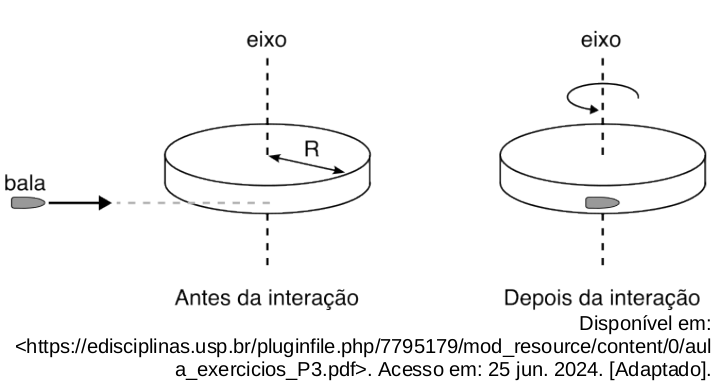
\includegraphics[width=0.8\textwidth]{figures/momento_angular.png}
\end{figure}

Uma bala de massa m se move horizontalmente com
velocidade v. A bala atinge a borda de um disco sólido, que
está inicialmente em repouso, ficando cravada nele (ver a
figura). O disco tem massa M, raio R, momento de inércia
$MR^{2}/2$ e está livre para girar em torno de seu eixo. Qual é a
velocidade angular do disco imediatamente após a bala ser
cravada nele?

\begin{itemize}
\item[(A)] $\Huge \omega = \frac{Mv}{(m+\frac{M}{2})R}$
\item[(B)] $\Huge \omega = \frac{mv}{(m+\frac{M}{2})R}$
\item[(C)] $\Huge \omega = \frac{mv}{(\frac{M}{2}-m)R}$
\item[(D)] $\Huge \omega = \frac{Mv}{(\frac{M}{2}-m)R}$
\end{itemize}

\vspace{0.5cm}

\textcolor{red}{\textbf{Solução:}}\\

\textbf{Princípio:}  
Como não há torques externos atuando em torno do eixo vertical, o momento angular do sistema em relação ao eixo é conservado.

\subsubsection*{Antes da colisão}
O momento angular do sistema em torno do eixo é apenas devido à bala:
\[
L_{\text{inicial}} = m v R
\]

\subsubsection*{Depois da colisão}
Após a colisão, a bala fica presa ao disco na borda, e o sistema (disco + bala) gira com velocidade angular \(\omega\).

Momento angular do disco:
\[
L_{\text{disco}} = I_{\text{disco}} \cdot \omega = \frac{1}{2} M R^2 \cdot \omega
\]

Momento angular da bala (considerada puntiforme a distância \(R\) do eixo):
\[
L_{\text{bala}} = m R^2 \cdot \omega
\]

Assim, o momento angular total após a colisão é:
\[
L_{\text{final}} = \left( \frac{1}{2} M R^2 + m R^2 \right) \omega
\]

\subsubsection*{Conservação do momento angular}
\[
L_{\text{inicial}} = L_{\text{final}}
\]

\[
m v R = \left( \frac{1}{2} M R^2 + m R^2 \right) \omega
\]

Dividindo ambos os lados por \(R\):
\[
m v = \left( \frac{1}{2} M + m \right) R \omega
\]

Isolando \(\omega\):
\[
\omega = \frac{m v}{R \left( \frac{1}{2} M + m \right)}
\]

\subsection*{Resposta final:}
\[
\boxed{
\omega = \frac{m v}{\left(m + \frac{1}{2} M\right)R}
}
\]

A resposta correta é alternativa \colorbox{green!50}{\textbf{B}}.
\end{flushleft}

\noindent\rule{\linewidth}{0.6pt}\\

\begin{flushleft}
\textbf{\textcolor{blue}{\Large Q38}}\\
\noindent
\colorbox{green!30}{Qual o astrônomo que propôs um modelo geocêntrico que
permitia descrever e prever} \colorbox{green!30}{as posições dos planetas e que, para isso, propôs que o movimento retrógrado dos planetas}
não tem sempre o mesmo aspecto e duração?

\begin{itemize}
\item[(A)] Galileu Galilei.
\item[(B)] Johannes Kepler.
\item[(C)] Cláudio Ptolomeu.
\item[(D)] Nicolau Copérnico.
\end{itemize}

\vspace{0.5cm}

\textcolor{red}{\textbf{Solução:}}\\

\section*{Resposta correta}

\[
\boxed{\text{(C) Cláudio Ptolomeu}}
\]

\section*{Explicação detalhada}

\subsection*{Quem foi Ptolomeu?}
Cláudio Ptolomeu foi um astrônomo, matemático e geógrafo grego que viveu em Alexandria, no Egito, no século II d.C. Ele escreveu a obra \textit{Almagesto}, que se tornou o principal tratado astronômico da Antiguidade e da Idade Média.

\subsection*{O que ele propôs?}
Ptolomeu refinou o antigo modelo geocêntrico (originalmente defendido por Aristóteles e Hiparco), criando um sistema geométrico e matemático capaz de:
\begin{itemize}
    \item Prever com precisão a posição dos planetas no céu em diferentes datas.
    \item Explicar por que os planetas às vezes parecem parar e andar para trás (\textit{movimento retrógrado aparente}).
\end{itemize}

\subsection*{Como ele explicou o movimento retrógrado?}
Para explicar o movimento retrógrado no \textbf{modelo geocêntrico}, Ptolomeu propôs que cada planeta não girava apenas em torno da Terra, mas fazia isso percorrendo duas trajetórias ao mesmo tempo:
\begin{itemize}
    \item Um \textbf{deferente}: círculo grande ao redor da Terra.
    \item Um \textbf{epiciclo}: círculo menor, cujo centro se move ao longo do deferente.
\end{itemize}

Esse sistema (\textit{deferente + epiciclo}) conseguia reproduzir as irregularidades do movimento dos planetas, inclusive o fato de que o movimento retrógrado não tinha sempre o mesmo tamanho nem a mesma duração para cada planeta.

\section*{Por que não as outras alternativas?}

\begin{itemize}
    \item \textbf{(A) Galileu Galilei}: Defendeu o heliocentrismo e fez observações com telescópio (\textit{séc. XVII}).
    \item \textbf{(B) Johannes Kepler}: Refinou o heliocentrismo com órbitas elípticas, rejeitando o geocentrismo (\textit{séc. XVII}).
    \item \textbf{(D) Nicolau Copérnico}: Propôs o heliocentrismo com órbitas circulares (\textit{séc. XVI}).
\end{itemize}

Somente \textbf{Ptolomeu} defendeu um modelo \textbf{geocêntrico}, consistente com as crenças da época, que já explicava as variações do movimento retrógrado.

\section*{Resumo}

\begin{center}
\small
\begin{tabular}{|c|c|c|}
\hline
\textbf{Astrônomo} & \textbf{Modelo} & \textbf{Movimento retrógrado} \\
\hline
\textbf{Ptolomeu} & Geocêntrico com epiciclos & Explicava corretamente o aspecto variável \\
\hline
Galileu & Heliocentrismo com telescópio & Observações em defesa do heliocentrismo \\
\hline
Kepler & Heliocentrismo com órbitas elípticas & Refinamento matemático \\
\hline
Copérnico & Heliocentrismo com órbitas circulares & Proposta inicial \\
\hline
\end{tabular}
\end{center}


A resposta correta é alternativa \colorbox{green!50}{\textbf{C}}.
\end{flushleft}

\noindent\rule{\linewidth}{0.6pt}\\

\section*{Gravitação Universal}

\textbf{Lei da Gravitação Universal:}
\begin{equation*}
  F = -G \frac{m_1 m_2}{r^2}
\end{equation*}

\textbf{Campo gravitacional:}
\begin{equation*}
  g = \frac{G M}{r^2}
\end{equation*}

\textbf{Energia potencial gravitacional:}
\begin{equation*}
  E_p = -\frac{G M m}{r}
\end{equation*}

\section*{Demonstração da Velocidade de Escape}

\colorbox{green!40}{A velocidade de escape é a mínima velocidade necessária para um corpo escapar da} \\
\colorbox{green!40}{gravidade de um planeta,} sem considerar resistência do ar.

\subsection*{Conservação de Energia}

Considerando um corpo de massa $m$ lançado da superfície de um planeta de massa $M$ e raio $R$:

\begin{itemize}
  \item Energia mecânica inicial:
  \[
  E_{\text{inicial}} = \frac{1}{2}mv^{2}_{e} - \frac{GMm}{R}
  \]
  \item Energia mecânica final (no infinito): 
  \[
  E_{\text{final}} = 0
  \]
\end{itemize}

Aplicando a conservação da energia:

\[
\frac{1}{2}mv^2_{e} - \frac{GMm}{R} = 0
\Rightarrow \frac{1}{2}v^2_{e} = \frac{GM}{R}
\Rightarrow v_{e} = \sqrt{\frac{2GM}{R}}
\]

\noindent
\textbf{Conclusão:} A velocidade de escape depende apenas da massa e do raio do corpo celeste, e não da massa do objeto lançado.

\noindent\rule{\linewidth}{0.6pt}\\

\begin{flushleft}
\textbf{\textcolor{blue}{\Large Questao 38}}\\
\noindent
Um foguete é lançado verticalmente para cima a partir da
superfície da Terra. Se a velocidade inicial do foguete for
metade da velocidade de escape da Terra, qual a altura que
o foguete atingirá, em unidades do raio da Terra (R$_{T}$)?
Despreze as influências da rotação da Terra no movimento
do foguete.

\begin{itemize}
\item[(A)] (7/3)R$_{T}$.
\item[(B)] (5/3)R$_{T}$.
\item[(C)] (2/3)R$_{T}$.
\item[(D)] (1/3)R$_{T}$.
\end{itemize}

\vspace{0.5cm}

\textcolor{red}{\textbf{Solução:}}\\

A energia mecânica total do foguete se conserva, pois desprezamos a resistência do ar.  
Na superfície da Terra (\(r = R_T\)), a energia total é a soma da energia cinética e potencial:  

\[
E_i = \frac{1}{2} m v_0^2 - \frac{G M_T m}{R_T}
\]

Na altura máxima (\(r = r_{\text{max}}\)), a velocidade do foguete é nula (\(v_f = 0\)):  

\[
E_f = 0 - \frac{G M_T m}{r_{\text{max}}}
\]

Conservação da energia mecânica: \(E_i = E_f\)  
Portanto:

\[
\frac{1}{2} m v_0^2 - \frac{G M_T m}{R_T} = - \frac{G M_T m}{r_{\text{max}}}
\]

Cancelamos \(m\) em todos os termos:

\[
\frac{1}{2} v_0^2 - \frac{G M_T}{R_T} = - \frac{G M_T}{r_{\text{max}}}
\]

Sabemos que a \textbf{velocidade de escape} é dada por:

\[
v_e = \sqrt{\frac{2 G M_T}{R_T}}
\]

Como a velocidade inicial do foguete é \(v_0 = \frac{v_e}{2}\), temos:

\[
v_0^2 = \left( \frac{v_e}{2} \right)^2 = \frac{v_e^2}{4} = \frac{1}{4} \cdot \frac{2 G M_T}{R_T} = \frac{G M_T}{2 R_T}
\]

Substituímos \(v_0^2\) na equação da energia:

\[
\frac{1}{2} \cdot \frac{G M_T}{2 R_T} - \frac{G M_T}{R_T} = - \frac{G M_T}{r_{\text{max}}}
\]

\[
\frac{G M_T}{4 R_T} - \frac{G M_T}{R_T} = - \frac{G M_T}{r_{\text{max}}}
\]

\[
-\frac{3}{4} \cdot \frac{G M_T}{R_T} = - \frac{G M_T}{r_{\text{max}}}
\]

Eliminamos o sinal e \(G M_T\):

\[
\frac{3}{4 R_T} = \frac{1}{r_{\text{max}}}
\]

Então:

\[
r_{\text{max}} = \frac{4}{3} R_T
\]

A altura máxima \(h_{\text{max}}\) acima da superfície é:

\[
h_{\text{max}} = r_{\text{max}} - R_T = \frac{4}{3} R_T - R_T = \frac{1}{3} R_T
\]

\section*{Resposta final:}

\[
\boxed{h_{\text{max}} = \frac{1}{3} R_T}
\]

O foguete atinge uma altura máxima igual a \(\frac{1}{3}\) do raio da Terra.


A resposta correta é alternativa \colorbox{green!50}{\textbf{D}}.
\end{flushleft}

\noindent\rule{\linewidth}{0.6pt}\\

\begin{flushleft}
\textbf{\textcolor{blue}{\Large Q39}}\\
\noindent
Um satélite de massa m orbita um planeta de massa M em
uma órbita circular de raio R. O tempo necessário para uma
volta completa do satélite em torno do planeta é

\begin{itemize}
\item[(A)] independente de M.
\item[(B)] proporcional a R$^{3/2}$.
\item[(C)] dependente de m.
\item[(D)] proporcional a R$^{2}$.
\end{itemize}

\vspace{0.5cm}

\textcolor{red}{\textbf{Solução:}}\\

A força gravitacional fornece a força centrípeta necessária:

\[
\frac{G M m}{R^2} = m \frac{v^2}{R}
\]

Cancelando \(m\) e resolvendo para \(v\):

\[
v = \sqrt{\frac{G M}{R}}
\]

O período \(T\) é dado por:

\[
T = \frac{2\pi R}{v}
\]

Substituindo \(v\):

\[
T =
\sqrt{\frac{4 \pi^{2} R^{3}}{G M}} =\sqrt{\frac{4 \pi^{2}}{G M}}\sqrt{R^{3}} = \sqrt{\frac{4 \pi^{2}}{G M}} R^{3/2}
\]


\section*{Resposta final:}

\[
\boxed{
T \propto R^{3/2}
}
\]


A resposta correta é alternativa \colorbox{green!50}{\textbf{B}}.
\end{flushleft}

\noindent\rule{\linewidth}{0.6pt}\\

\begin{flushleft}
\textbf{\textcolor{blue}{\Large Q40}}\\
\noindent
Uma função de estado de um sistema termodinâmico fica
completamente definida quando o estado do sistema é
especificado. Isso pode ser representado num diagrama
pressão-volume do sistema, que ilustra seus estados inicial
e final. Qual das grandezas abaixo é uma função de estado
de um sistema termodinâmico?

\begin{itemize}
\item[(A)] A energia interna.
\item[(B)] O calor.
\item[(C)] O trabalho.
\item[(D)] A massa.
\end{itemize}

\vspace{0.5cm}

\textcolor{red}{\textbf{Solução:}}\\

\section*{Introdução: Funções de Estado em Termodinâmica}

A Termodinâmica é a área da Física que estuda as transformações de energia e as propriedades macroscópicas da matéria, como temperatura, pressão e volume. Para descrever um sistema termodinâmico, é necessário especificar o \textbf{estado do sistema}, que é determinado por um conjunto de variáveis chamadas \textbf{variáveis de estado}.

Quando um sistema evolui de um estado inicial para um estado final, podemos calcular as mudanças sofridas em algumas grandezas físicas. Algumas dessas grandezas dependem apenas do estado inicial e final do sistema, enquanto outras dependem do caminho seguido durante o processo.

\subsection*{O que é uma função de estado?}

Uma \textbf{função de estado} é uma grandeza física cujo valor só depende do estado atual do sistema, isto é, das condições termodinâmicas (como \(P\), \(V\), \(T\), \(U\) etc.), e \textbf{não depende do processo pelo qual o sistema chegou a esse estado}.

Ou seja:
\begin{quote}
As funções de estado são propriedades macroscópicas que caracterizam completamente o estado do sistema. Sua variação entre dois estados é a mesma, independentemente do caminho percorrido entre eles.
\end{quote}

\subsection*{Exemplos clássicos de funções de estado:}
\begin{itemize}
    \item Energia interna (\(U\))
    \item Entalpia (\(H\))
    \item Entropia (\(S\))
    \item Pressão (\(P\))
    \item Volume (\(V\))
    \item Temperatura (\(T\))
\end{itemize}

Essas grandezas podem ser representadas em diagramas, como os famosos diagramas \(P \times V\) ou \(T \times S\), que ilustram estados e trajetórias de processos.

\subsection*{E o que não é função de estado?}

Grandezas como o \textbf{calor trocado} (\(Q\)) e o \textbf{trabalho realizado} (\(W\)) durante um processo dependem de 
como o sistema evoluiu — são chamadas de \textbf{funções de processo}.

Por exemplo: para comprimir um gás do volume \(V_1\) ao volume \(V_2\), o trabalho realizado pode ser maior ou menor 
dependendo do caminho seguido (isotérmico, adiabático etc.), mas a variação de energia interna só depende do estado inicial e final.

A resposta correta é alternativa \colorbox{green!50}{\textbf{A}}.
\end{flushleft}

\noindent\rule{\linewidth}{0.6pt}\\

\begin{flushleft}
\textbf{\textcolor{blue}{\Large Q41}}\\
\noindent
Uma bomba de calor serve para extrair calor do ambiente
externo a 7°C e aquecer o interior de uma casa a 27°C.
Considerando que a bomba é uma máquina de Carnot, para
cada 15.000 J de calor entregue dentro de casa, a menor
quantidade de trabalho que deve ser fornecido à bomba é

\begin{itemize}
\item[(A)] 2.500 J.
\item[(B)] 2.000 J.
\item[(C)] 1.500 J.
\item[(D)] 1.000 J.
\end{itemize}

\vspace{0.5cm}

\textcolor{red}{\textbf{Solução:}}\\

\section*{Definição}

Uma máquina térmica converte calor em trabalho, operando entre duas fontes térmicas.

\section*{Rendimento}

\[
\eta = \frac{W}{Q_q} = \frac{Q_q - Q_f}{Q_q} = 1 - \frac{Q_f}{Q_q}
\]

\begin{itemize}
  \item \( \eta \): rendimento
  \item \( W \): trabalho útil
  \item \( Q_q \): calor absorvido da fonte quente
  \item \( Q_f \): calor rejeitado à fonte fria
\end{itemize}

\section*{Rendimento da Máquina de Carnot}

\[
\eta_{\text{Carnot}} = 1 - \frac{T_f}{T_q}
\]

\subsection*{Calcular o rendimento da bomba de calor:}

\[
\eta = 1 - \frac{T_f}{T_q} = 1 - \frac{7^{\circ}\textrm{C} + 273\textrm{K}}{27^{\circ}\textrm{C}+ 273\textrm{K}} = 1 - \frac{280}{300} = 1 - 0.933333 = 0.066667 = 6.67\%
\]

Agora podemos calcular o trabalho realizado pela bomba de calor:

\[
  W = \eta Q_q = 6.67\% \times 15.000 \textrm{J} = 1.000 \textrm{J}
\]
A resposta correta é alternativa \colorbox{green!50}{\textbf{D}}.
\end{flushleft}

\noindent\rule{\linewidth}{0.6pt}\\

\section*{Princ\'ipios da Termodinâmica}

\subsection*{Primeiro Princípio}
\begin{equation*}
    \Delta U = Q - W   \hspace{0.5cm} \longrightarrow \hspace{0.5cm} Q = W + \Delta U
\end{equation*}
\subsection*{Segundo Princípio}
\begin{itemize}
    \item O calor não flui espontaneamente de um corpo frio para um corpo quente.
    \item Entropia tende a aumentar.
\end{itemize}

\section*{O que é entropia?}
A entropia (\(S\)) é uma função de estado que mede o grau de desordem de um sistema, a quantidade de microestados possíveis, e a irreversibilidade de processos.

\section*{Definição termodinâmica}
Para processos reversíveis:

\[
\Delta S = \int \frac{dQ_{\text{rev}}}{T}
\]

Para temperatura constante (isotérmico):

\[
\Delta S = \frac{Q_{\text{rev}}}{T}
\]

\section*{Segunda Lei da Termodinâmica}

\[
\Delta S_{\text{total}} \geq 0
\]

\begin{itemize}
  \item \( \Delta S_{\text{total}} = 0 \): processo reversível
  \item \( \Delta S_{\text{total}} > 0 \): processo irreversível
\end{itemize}

\section*{Entropia estatística (Boltzmann)}

\[
S = k_B \ln \Omega
\]

\begin{itemize}
  \item \( k_B = 1{,}38 \times 10^{-23} \, \text{J/K} \)
  \item \( \Omega \): número de microestados possíveis
\end{itemize}

\section*{Unidade}
Joules por Kelvin (J/K)

\section*{Exemplos onde a entropia aumenta}
\begin{itemize}
  \item Derretimento de gelo
  \item Expansão de gás
  \item Mistura de substâncias
\end{itemize}

\subsection*{Terceiro Princípio}
\begin{itemize}
    \item A entropia de um cristal perfeito é zero no zero absoluto $(0\,K)$.
\end{itemize}

\noindent\rule{\linewidth}{0.6pt}\\

\begin{flushleft}
\textbf{\textcolor{blue}{\Large Q42}}\\
\noindent
Um corpo de massa m com calor específico C à temperatura
de 500 K é colocado em contato com outro corpo de mesma
massa e mesmo calor específico à temperatura de 100 K. O
sistema é colocado dentro de uma caixa isolada
termicamente durante o processo. A variação da entropia do
sistema quando os blocos alcançam o equilíbrio térmico é

\begin{itemize}
\item[(A)] mCln 5.
\item[(B)] mCln 3.
\item[(C)] mCln(9/5).
\item[(D)] mCln(5/3).
\end{itemize}

\vspace{0.5cm}

\textcolor{red}{\textbf{Solução:}}\\

\section*{Variação de Entropia do Sistema}

\textbf{Dados do problema:}
\begin{itemize}
    \item Dois corpos idênticos: mesma massa \(m\) e mesmo calor específico \(C\)
    \item Temperatura inicial do corpo quente: \(T_q = 500\,\mathrm{K}\)
    \item Temperatura inicial do corpo frio: \(T_f = 100\,\mathrm{K}\)
    \item Caixa isolada termicamente (processo adiabático para o universo, mas irreversível para o sistema)
\end{itemize}

Queremos calcular a variação de entropia do sistema quando os corpos atingem o equilíbrio térmico.

\subsection*{Temperatura de equilíbrio}

Como os corpos têm mesma massa e mesmo calor específico, a energia perdida pelo quente é igual à energia ganha pelo frio. Assim, a temperatura de equilíbrio é a média aritmética:
\[
T_e = \frac{T_q + T_f}{2} = \frac{500 + 100}{2} = 300\,\mathrm{K}
\]

\subsection*{Variação de entropia de cada corpo}

Sabemos que a variação de entropia de um corpo com calor específico constante é dada por:
\[
\Delta S = mC \int_{T_i}^{T_f} \frac{dT}{T} = mC \ln\left( \frac{T_f}{T_i} \right)
\]

\textbf{Para o corpo quente:}
\[
\Delta S_q =
mC \ln\left( \frac{T_e}{T_q} \right) =
mC \ln\left( \frac{300}{500} \right) =
mC \ln(0{,}6)
\]

\textbf{Para o corpo frio:}
\[
\Delta S_f =
mC \ln\left( \frac{T_e}{T_f} \right) =
mC \ln\left( \frac{300}{100} \right) =
mC \ln(3)
\]

\subsection*{Variação de entropia total do sistema}

A variação de entropia total do sistema é a soma das variações de cada corpo:
\[
\Delta S_\text{total} =
\Delta S_q + \Delta S_f =
mC \ln(0{,}6) + mC \ln(3)
\]

Utilizando a propriedade dos logaritmos:
\[
\ln(0{,}6) + \ln(3) = \ln(0{,}6 \times 3) = \ln(1{,}8)
\]

Logo:
\[
\Delta S_\text{total} =
mC \ln(\frac{9}{5})
\]

\subsection*{Resposta final:}
\[
\boxed{
\Delta S_\text{total} =
mC \ln(\frac{9}{5})
}
\]



A resposta correta é alternativa \colorbox{green!50}{\textbf{C}}.
\end{flushleft}

\noindent\rule{\linewidth}{0.6pt}\\

\section*{Condições para Interferência em Filmes Finos (Incidência Normal)}

Quando a luz incide perpendicularmente a um filme fino de espessura \( d \) e índice de refração \( n \), a diferença 
de caminho óptico entre os dois feixes refletidos é:

\[
\Delta = 2nd
\]

A condição de interferência depende da ocorrência (ou não) de inversão de fase ao refletir nas interfaces. 

\subsection*{Interferência Construtiva}

\begin{itemize}
  \item \textbf{Com inversão de fase em uma das interfaces:}
  \[
  2nd = \left( m + \frac{1}{2} \right) \lambda
  \]
  
  \item \textbf{Sem inversão de fase (ou inversão em ambas):}
  \[
  2nd = m \lambda
  \]
\end{itemize}

\subsection*{Interferência Destrutiva}

\begin{itemize}
  \item \textbf{Com inversão de fase em uma das interfaces:}
  \[
  2nd = m \lambda
  \]
  
  \item \textbf{Sem inversão de fase (ou inversão em ambas):}
  \[
  2nd = \left( m + \frac{1}{2} \right) \lambda
  \]
\end{itemize}

\noindent Onde:
\begin{itemize}
  \item \( n \) é o índice de refração do filme;
  \item \( d \) é a espessura do filme;
  \item \( \lambda \) é o comprimento de onda da luz no ar;
  \item \( m \in \mathbb{Z} \) é a ordem da interferência.
\end{itemize}

\noindent\rule{\linewidth}{0.6pt}\\

\begin{flushleft}
\textbf{\textcolor{blue}{\Large Q43}}\\
\noindent
Luz com 650 nm de comprimento de onda incide
perpendicularmente em um filme fino de sabão, que tem
índice de refração igual a 1,30. Sabendo que esse filme está
suspenso no ar, qual a menor espessura que esse filme
deve ter para que as ondas refletidas por ele sofram
interferência construtiva?

\begin{itemize}
\item[(A)] 320 nm.
\item[(B)] 242 nm.
\item[(C)] 125 nm.
\item[(D)] 117 nm.
\end{itemize}

\vspace{0.5cm}

\textcolor{red}{\textbf{Solução:}}\\

\section*{Interferência construtiva em um filme de sabão}

\textbf{Dados:}
\begin{itemize}
    \item Comprimento de onda no ar: \( \lambda_0 = 650\,\mathrm{nm} \)
    \item Índice de refração do filme: \( n_f = 1{,}30 \)
    \item Índice de refração do ar: \( n_{ar} \approx 1 \)
\end{itemize}

O filme está suspenso no ar. Queremos a menor espessura \(e\) para que a luz refletida tenha interferência construtiva.

\subsection*{Condição de fase}

Quando a luz incide sobre a superfície do filme:
\begin{itemize}
    \item Na interface ar–sabão (\(n_\text{ar} < n_\text{sabão}\)), ocorre inversão de fase de \(\pi\) (equivalente a \(\lambda/2\)).
    \item Na interface sabão–ar (\(n_\text{sabão} > n_\text{ar}\)), não ocorre inversão.
\end{itemize}

Como há uma inversão de fase, a condição para \textbf{interferência construtiva} é:
\[
2e = \left(m + \frac{1}{2}\right) \lambda_f
\]

Para a menor espessura (\(m = 0\)):
\[
2e = \frac{\lambda_f}{2} \quad \implies \quad e = \frac{\lambda_f}{4}
\]

\subsection*{Comprimento de onda no filme}

No interior do filme, o comprimento de onda é menor:
\[
\lambda_f = \frac{\lambda_0}{n_f} = \frac{650}{1{,}30} \approx 500\,\mathrm{nm}
\]

\subsection*{Espessura mínima}

Substituindo:
\[
e_\text{mín} = \frac{\lambda_f}{4} = \frac{500}{4} = 125\,\mathrm{nm}
\]

\subsection*{Resposta final:}
\[
\boxed{e_\text{mín} = 125\,\mathrm{nm}}
\]


A resposta correta é alternativa \colorbox{green!50}{\textbf{C}}.
\end{flushleft}

\noindent\rule{\linewidth}{0.6pt}\\

\section*{Intervalo válido para o comprimento de onda de um laser}

O comprimento de onda (\( \lambda \)) de um laser depende do material ativo utilizado no laser e pode abranger diferentes regiões do espectro eletromagnético. Abaixo estão os intervalos típicos para lasers comuns:

\begin{center}
\begin{tabular}{|l|c|}
\hline
\textbf{Tipo de laser} & \textbf{Comprimento de onda (\( \lambda \))} \\
\hline
Laser ultravioleta (UV) & \(180\,\mathrm{nm} \text{ a } 400\,\mathrm{nm}\) \\
\hline
Laser visível (vermelho–violeta) & \(400\,\mathrm{nm} \text{ a } 700\,\mathrm{nm}\) \\
\hline
Laser infravermelho próximo (NIR) & \(700\,\mathrm{nm} \text{ a } 1400\,\mathrm{nm}\) \\
\hline
Laser infravermelho médio & \(1400\,\mathrm{nm} \text{ a } 3000\,\mathrm{nm}\) \\
\hline
Laser infravermelho distante & \(>3000\,\mathrm{nm}\) \\
\hline
\end{tabular}
\end{center}

\vspace{0.5cm}

\subsection*{Exemplos comuns de lasers visíveis:}
\begin{itemize}
    \item Laser vermelho (He-Ne ou diodo): \(630\,\mathrm{nm} – 680\,\mathrm{nm}\)
    \item Laser verde (Nd:YAG com dobro da frequência): \(532\,\mathrm{nm}\)
    \item Laser azul: \(405\,\mathrm{nm} – 488\,\mathrm{nm}\)
    \item Laser violeta: \( \sim 400\,\mathrm{nm} \)
\end{itemize}

\vspace{0.5cm}

Para lasers visíveis, o intervalo típico de comprimento de onda válido é aproximadamente:
\[
\boxed{400\,\mathrm{nm} \leq \lambda \leq 700\,\mathrm{nm}}
\]

\begin{flushleft}
\textbf{\textcolor{blue}{\Large Q44}}\\
\noindent
Um feixe de luz laser incide sobre uma fenda estreita, e uma
figura de difração é observada sobre uma tela localizada a 5,0 m
da fenda. A distância vertical entre o centro do primeiro mínimo
acima do máximo central e o centro do primeiro mínimo abaixo
do máximo central é de 20 mm. Qual é a largura da fenda?

\begin{itemize}
\item[(A)] 0,30 mm.
\item[(B)] 0,45 mm.
\item[(C)] 0,55 mm.
\item[(D)] 0,65 mm.
\end{itemize}

\vspace{0.5cm}

\textcolor{red}{\textbf{Solução:}}\\

\subsection*{Passo 1: Condição para os mínimos}

Para uma fenda simples, os mínimos ocorrem em ângulos \(\theta\) tais que:
\[
a \cdot \sin\theta = m\lambda
\]
Para o primeiro mínimo (\(m=1\)):
\[
\sin\theta_1 = \frac{\lambda}{a}
\]

\vspace{0.5cm}

\subsection*{Passo 2: Relação geométrica na tela}

Na tela, a distância vertical entre o máximo central e o primeiro mínimo é aproximadamente:
\[
y_1 = L \cdot \tan\theta_1 \approx L \cdot \sin\theta_1
\]

A distância total entre o primeiro mínimo acima e o primeiro mínimo abaixo é:
\[
\Delta y = 2y_1
\]

Substituindo \(y_1\):
\[
\Delta y = 2L \cdot \sin\theta_1
\]

E como \(\sin\theta_1 = \lambda/a\):
\[
\Delta y = 2L \cdot \frac{\lambda}{a}
\]

\vspace{0.5cm}

\subsection*{Passo 3: Resolvendo para \(a\)}

Isolando \(a\):
\[
a = 2L \cdot \frac{\lambda}{\Delta y}
\]

Substituindo os valores numéricos:
\[
a = 2 \cdot 5{,}0 \cdot \frac{6{,}5 \times 10^{-7}}{0{,}020}
\]

\[
a = 10{,}0 \cdot 3{,}25 \times 10^{-5} = 3{,}25 \times 10^{-4}\,m
\]

Convertendo para milímetros:
\[
a = 0{,}325\,mm
\]

\vspace{0.5cm}

\subsection*{Resposta final:}

\[
\boxed{a \approx 0{,}325\,mm}
\]

A resposta correta é alternativa \colorbox{green!50}{\textbf{A}}.
\end{flushleft}

\noindent\rule{\linewidth}{0.6pt}\\

\begin{flushleft}
\textbf{\textcolor{blue}{\Large Q45 }}\\
\noindent
Uma rede de difração possui \( 1{,}25 \times 10^{4} \) fendas uniformemente espaçadas, de forma que a largura total da rede é \( 25,0\,\mathrm{mm} \).  
Determine o ângulo \( \theta \) correspondente ao máximo de primeira ordem.

\begin{itemize}
\item[(A)] $4{,}35 \times 10^{-4} \textrm{ rad/nm}$.
\item[(B)] $5{,}26 \times 10^{-4} \textrm{ rad/nm}$.
\item[(C)] $3{,}87 \times 10^{-4} \textrm{ rad/nm}$.
\item[(D)] $2{,}19 \times 10^{-4} \textrm{ rad/nm}$.
\end{itemize}

\vspace{0.5cm}

\textcolor{red}{\textbf{Solução:}}\\

\subsection*{Dados:}
\begin{itemize}
    \item Número de fendas: \( N = 1{,}25 \times 10^4 \)
    \item Largura da rede: \( L = \SI{25,0}{mm} = 25,0 \times 10^{-3}\,\mathrm{m} \)
    \item Ordem do máximo: \( m = 1 \)
\end{itemize}

\subsection*{Passo 1: Condição para o máximo de difração}

Para um máximo de ordem \(m\), a condição de difração é:
\[
d \, \sin\theta = m\lambda
\]

Para \(m=1\) e pequenos ângulos (\( \sin\theta \approx \theta \)):
\[
\theta \approx \frac{\lambda}{d}
\]

Logo, a razão \( \theta/\lambda \) é:
\[
\frac{\theta}{\lambda} \approx \frac{1}{d}
\]

\subsection*{Passo 2: Espaçamento entre as fendas}

O espaçamento \(d\) entre fendas é dado por:
\[
d = \frac{L}{N}
\]

Substituindo os valores:
\[
d = \frac{25{,}0 \times 10^{-3}}{1{,}25 \times 10^4} = 2{,}0 \times 10^{-6}\,\mathrm{m}
\]

\subsection*{Passo 3: Calculando \( \theta/\lambda \)}

Em \(\mathrm{m}^{-1}\):
\[
\frac{\theta}{\lambda} = \frac{1}{2{,}0 \times 10^{-6}} = 5{,}0 \times 10^{5}\,\mathrm{m}^{-1}
\]

Convertendo para \(\mathrm{nm}^{-1}\), sabendo que \(1\,\mathrm{m} = 10^{9}\,\mathrm{nm}\):
\[
\frac{\theta}{\lambda} = 5{,}0 \times 10^{5} \times 10^{-9} = 5{,}0 \times 10^{-4}\,\mathrm{rad/nm}
\]

O valor mais próximo entre as alternativas é:
\[
\boxed{\frac{\theta}{\lambda} = 5{,}26 \times 10^{-4}\,\mathrm{rad/nm}}
\]


A resposta correta é alternativa \colorbox{green!50}{\textbf{B}}.
\end{flushleft}

\noindent\rule{\linewidth}{0.6pt}\\

\begin{flushleft}
\textbf{\textcolor{blue}{\Large Q46}}\\
\noindent
Um pesquisador que está estudando a propagação de ondas em uma corda observa a seguinte situação: uma
onda estacionária se forma na corda, com nós (pontos de amplitude zero) a cada 0,5 m, amplitude de 2,0 m e
velocidade de propagação de 2,0 m/s. A equação que o pesquisador obtém para descrever a onda estacionária é

\begin{itemize}
\item[(A)] $y(x,t) = 2\sin(\pi x)\cos(4\pi t)$
\item[(B)] $y(x,t) = 2\sin(2\pi x)\cos(4\pi t)$
\item[(C)] $y(x,t) = 2\sin(2\pi x)\cos(\pi t)$
\item[(D)] $y(x,t) = 2\sin(\pi x)\cos(\pi t)$
\end{itemize}

\vspace{0.5cm}

\textcolor{red}{\textbf{Solução:}}\\

\textbf{Resolução:}

\bigskip

\textbf{Dados do problema:}
\begin{itemize}
    \item Distância entre nós consecutivos: \(0{,}5\,m\)
    \item Amplitude máxima: \(A = 2,0\,m\)
    \item Velocidade de propagação: \(v = 2,0\,m/s\)
\end{itemize}

Queremos encontrar a equação da onda estacionária no formato:
\[
y(x,t) = 2A \sin(kx) \cos(\omega t)
\]

Sabemos que o fator \(2A\) já é dado como \(2,0\), então apenas precisamos determinar \(k\) e \(\omega\).

\bigskip

\textbf{Passo 1: distância entre nós}

Em uma onda estacionária, a distância entre dois nós consecutivos é igual a \(\lambda/2\).  
Como o problema informa que essa distância é \(0{,}5\,m\), temos:
\[
\frac{\lambda}{2} = 0{,}5 \quad \Longrightarrow \quad \lambda = 1,0\,m
\]

\bigskip

\textbf{Passo 2: número de onda \(k\)}

O número de onda é dado por:
\[
k = \frac{2\pi}{\lambda} = \frac{2\pi}{1,0} = 2\pi
\]

Portanto, o fator espacial da solução é \(\sin(2\pi x)\).

\bigskip

\textbf{Passo 3: frequência angular \(\omega\)}

Usamos a relação entre velocidade, frequência e comprimento de onda:
\[
v = \lambda f \quad \Longrightarrow \quad f = \frac{v}{\lambda} = \frac{2,0}{1,0} = 2,0\,Hz
\]

E como \(\omega = 2\pi f\), temos:
\[
\omega = 2\pi \cdot 2 = 4\pi
\]

\bigskip

\textbf{Passo 4: equação final}

Substituindo os valores encontrados:
\[
y(x,t) = 2 \sin(2\pi x) \cos(4\pi t)
\]

\bigskip

\textbf{Resposta correta:}
\[
\boxed{y(x,t) = 2 \sin(2\pi x) \cos(4\pi t)}
\]

Essa equação possui duas partes principais:

\bigskip

\textbf{Parte espacial:} \(\sin(kx)\)
\begin{itemize}
    \item Determina o padrão fixo de \textbf{nós} (onde a amplitude é sempre zero) e \textbf{ventres} (onde a amplitude é máxima).
    \item Define a forma da onda ao longo do espaço.
\end{itemize}

\bigskip

\textbf{Parte temporal:} \(\cos(\omega t)\)
\begin{itemize}
    \item Descreve a oscilação harmônica no tempo.
    \item Cada ponto vibra com a frequência angular \(\omega\), mas com amplitude espacialmente determinada.
\end{itemize}


A resposta correta é alternativa \colorbox{green!50}{\textbf{B}}.
\end{flushleft}

\noindent\rule{\linewidth}{0.6pt}\\

\begin{flushleft}
\textbf{\textcolor{blue}{\Large Q47}}\\
\noindent

Duas fontes de ondas sonoras idênticas emitem ondas com
comprimento de onda de 0,5 m em fase. As fontes estão
separadas por uma distância de 1,5 m. Haverá interferência
construtiva ao longo da linha que liga as duas fontes nas
posições:

\begin{itemize}
\item[(A)] 0,25 m, 0,75 m, 1,25 m.
\item[(B)] 0,5 m, 1,0 m, 1,25 m.
\item[(C)] 0,5 m, 1,0 m, 1,5 m.
\item[(D)] 0,25 m, 0,5 m, 1,25 m.
\end{itemize}

\vspace{0.5cm}

\textcolor{red}{\textbf{Solução:}}\\

\colorbox{yellow!30}{A diferença de caminhos entre as ondas emitidas pelas duas fontes deve ser um múltiplo} 
\colorbox{yellow!30}{inteiro de \( \lambda \) para que ocorra \textbf{interferência construtiva}:}
\[
\Delta r = m\lambda, \quad m = 0, \pm1, \pm2, \dots
\]

Colocando as fontes nos pontos \( x=0 \) e \( x=d \), ao longo do eixo \( x \), temos para um ponto \( x \):
\[
\Delta r = |x - (d-x)| = |2x - d|
\]

Para interferência construtiva:
\[
2x - d = m\lambda
\]

Resolvendo para \( x \):
\[
x = \frac{d + m\lambda}{2}
\]

Substituindo \( d = 1{,}5 \) e \( \lambda = 0{,}5 \):
\[
x = \frac{1{,}5 + 0{,}5m}{2} = 0{,}75 + 0{,}25m
\]

Para que \( x \) esteja entre \( 0 \) e \( 1{,}5 \), os valores possíveis de \( m \) são \( m = -3, -2, -1, 0, 1, 2, 3 \), o que resulta nas posições:
\[
x = 0{,}0;\ 0{,}25;\ 0{,}5;\ 0{,}75;\ 1{,}0;\ 1{,}25;\ 1{,}5 \ \mathrm{m}
\]

Entre as alternativas dadas, a correta é:
\[
\boxed{\text{(A) } 0{,}25\,m,\ 0{,}75\,m,\ 1{,}25\,m}
\]


A resposta correta é alternativa \colorbox{green!50}{\textbf{A}}.
\end{flushleft}

\noindent\rule{\linewidth}{0.6pt}\\

\section*{Equilíbrio do Corpo Rígido e da Partícula}

\textbf{Condições de equilíbrio:}
\begin{align*}
  \sum \vec{F} &= 0 \quad \text{(equilíbrio translacional)} \\
  \sum \vec{\tau} &= 0 \quad \text{(equilíbrio rotacional)}
\end{align*}

\textbf{Torque (momento de uma força):}
\begin{equation*}
  \tau = r F \sin \theta
\end{equation*}

\begin{equation*}
  \vec{\tau} = \frac{d\vec{L}}{dt}
\end{equation*}

\begin{equation*}
  \tau = I.\alpha
\end{equation*}

\begin{equation*}
  \alpha = \frac{d^{2}\theta}{dt^{2}}
\end{equation*}

\begin{equation*}
  \frac{d^{2}\theta}{dt^{2}} + \frac{g}{L}\sin\theta = 0 \quad \textrm{MHS}
\end{equation*}

\begin{equation*}
  \frac{d^{2}\theta}{dt^{2}} + \omega^{2}\sin\theta = 0 \quad \textrm{MHS}
\end{equation*}

Solução geral EDO:
\begin{equation*}
  \theta(t) = \theta_{0} \cos(\omega t + \varphi)
\end{equation*}

\subsection*{Rota\c{c}\~ao de um Corpo R\'igido}
\begin{equation*}
  \omega = \frac{d\theta}{dt}, \quad \alpha = \frac{d\omega}{dt}
\end{equation*}

\begin{flushleft}
\textbf{\textcolor{blue}{\Large Q48}}\\
\noindent
Um pêndulo simples de comprimento \( L = 10\,m \) oscila com um ângulo máximo de oito graus \( 0{,}14\,\) rad.  
Considere a aceleração da gravidade \( g = 10\,\)m/s\(^2\). A equação diferencial que descreve o movimento do pêndulo para pequenos ângulos é dada por:
$\frac{d^2\theta}{dt^2} + \omega^2 \theta = 0$ sendo \( \omega \) a frequência angular do pêndulo e \( \theta \) o ângulo de deslocamento em função do tempo \( t \).  
Considerando as condições iniciais \( \theta(0) = \theta_0 \) e \( \frac{d\theta}{dt}(0) = 0 \), a solução geral da equação diferencial para o pêndulo é:

\begin{itemize}
\item[(A)] \( \theta(t) = 0{,}14\cos(0{,}1t) \).
\item[(B)] \( \theta(t) = 0{,}14\cos(0{,}4t) \).
\item[(C)] \( \theta(t) = 0{,}14\cos(0{,}8t) \).
\item[(D)] \( \theta(t) = 0{,}14\cos(t) \).
\end{itemize}

\vspace{0.5cm}

\textcolor{red}{\textbf{Solução:}}\\

\section*{Demonstração da equação do movimento do pêndulo simples a partir do torque}

Considere um pêndulo simples com comprimento \(L\) e massa \(m\), oscilando em torno do ponto de suspensão com um ângulo \(\theta(t)\) em relação à posição de equilíbrio vertical.

\bigskip

\textbf{1. Torque devido à força peso}

A força peso atua verticalmente para baixo com intensidade \(mg\). O torque em relação ao ponto de suspensão é:

\[
\boxed{\tau = - m g L \sin\theta,}
\]

onde o sinal negativo indica que o torque tende a restaurar o pêndulo para a posição de equilíbrio (\(\theta = 0\)).

\bigskip

\textbf{2. Momento de inércia do pêndulo simples}

Como o pêndulo é uma massa pontual no final de um fio de massa desprezível, o momento de inércia em relação ao ponto de suspensão é:

\[
\boxed{I = m L^2.}
\]

\bigskip

\textbf{3. Equação do movimento rotacional}

Aplicando a segunda lei de Newton para rotações, temos:

\[
\boxed{\tau = I \alpha,}
\]

onde \(\alpha = \frac{d^2 \theta}{dt^2}\) é a aceleração angular. Substituindo,

\[
- m g L \sin\theta = m L^2 \frac{d^2 \theta}{dt^2}.
\]

Dividindo ambos os lados por \(m L^2\):

\[
\boxed{\frac{d^2 \theta}{dt^2} + \frac{g}{L} \sin\theta = 0.}
\]

\bigskip

\textbf{4. Aproximação para pequenos ângulos}

Para pequenas oscilações, onde \(\theta \ll 1\) (rad), podemos aproximar \(\sin\theta \approx \theta\), obtendo a equação linearizada:

\[
\boxed{\frac{d^2 \theta}{dt^2} + \frac{g}{L} \theta = 0.}
\]

Definindo

\[
\omega = \sqrt{\frac{g}{L}},
\]

a equação diferencial torna-se

\[
\boxed{\frac{d^2 \theta}{dt^2} + \omega^2 \theta = 0.}
\]

\bigskip

\textbf{5. Solução da equação diferencial}

A solução geral da equação é

\[
\boxed{\theta(t) = A \cos(\omega t) + B \sin(\omega t),}
\]

onde as \colorbox{green!30}{constantes \(A\) e \(B\) são determinadas pelas condições iniciais.}

Dadas as condições:

\[
\theta(0) = \theta_0, \quad \frac{d\theta}{dt}(0) = 0,
\]

temos:

\[
\theta(0) = A = \theta_0,
\]

e

\[
\frac{d\theta}{dt} = - A \omega \sin(\omega t) + B \omega \cos(\omega t) \implies \frac{d\theta}{dt}(0) = B \omega = 0 \Rightarrow B = 0.
\]

Assim, a solução final é

\[
\theta(t) = \theta_0 \cos(\omega t) = \theta_0 \cos\left(\sqrt{\frac{g}{L}} \, t \right).
\]

\[
\boxed{
\theta(t) = \theta_0 \cos\left(\sqrt{\frac{10}{10}} \, t \right) = \theta_0 \cos\left(t \right).
}
\]

A resposta correta é alternativa \colorbox{green!50}{\textbf{D}}.
\end{flushleft}

\begin{flushleft}
\textbf{\textcolor{blue}{\Large Q49}}\\
\noindent
Considere uma região no espaço onde existe um campo elétrico variável no tempo, dado por $\vec{E} = E_0 \sin(\omega t) \, \hat{z},$
sendo \(E_0\) a amplitude do campo elétrico, \(\omega\) a frequência angular e \(t\) o tempo. De acordo com as equações de Maxwell, 
esse campo elétrico variável irá induzir um campo magnético também variável, dando origem a uma onda eletromagnética. Supondo que a 
onda eletromagnética se propague na direção \(+y\) e que não haja cargas livres ou correntes na região, a expressão que descreve o 
campo magnético \(B\) induzido nessa região é:


\begin{itemize}
\item[(A)] $B = \frac{ E_0}{c} \sin(\omega t) \, \hat{x}.$
\item[(B)] $B = -\frac{E_0}{c} \sin(\omega t) \, \hat{x}.$
\item[(C)] $B = \frac{E_0}{c} \cos(\omega t) \, \hat{x}.$
\item[(D)] $B = -\frac{E_0}{c} \cos(\omega t) \, \hat{x}.$
\end{itemize}

\vspace{0.5cm}

\textcolor{red}{\textbf{Solução:}}\\



\section*{1. Forma geral da onda eletromagnética no vácuo}

No vácuo, uma onda plana que se propaga na direção \(+\hat{y}\) tem os campos elétrico e magnético na forma:
\[
\vec{E}(y,t) = E_0 \sin(k y - \omega t) \, \hat{z},
\]
\[
\vec{B}(y,t) = B_0 \sin(k y - \omega t) \, \hat{x}.
\]

A relação entre as amplitudes \(E_0\) e \(B_0\) é dada por:
\[
B_0 = \frac{E_0}{c}.
\]

Considere a região do espaço onde o campo elétrico é dado por:
\[
\vec{E}(y,t) = E_0 \sin(k y - \omega t) \, \hat{z}.
\]

Queremos determinar o campo magnético associado \(\vec{B}(y,t)\), calculando o rotacional de \(\vec{E}\) e usando a \textbf{lei de Faraday}:
\[
\nabla \times \vec{E} = -\frac{\partial \vec{B}}{\partial t}.
\]

\section*{2. Cálculo do rotacional de \(\vec{E}\)}

O campo elétrico tem apenas a componente \(z\), que depende apenas de \(y\) e \(t\).  
Em coordenadas cartesianas:
\[
\nabla \times \vec{E} =
\begin{vmatrix}
\hat{x} & \hat{y} & \hat{z} \\[4pt]
\partial_x & \partial_y & \partial_z \\[4pt]
0 & 0 & E_z
\end{vmatrix}
=
\left( \frac{\partial E_z}{\partial y} \right) \hat{x} - \left( \frac{\partial E_z}{\partial x} \right) \hat{y} + 0 \, \hat{z}.
\]

Como \(E_z = E_0 \sin(k y - \omega t)\), temos:
\[
\frac{\partial E_z}{\partial y} = k E_0 \cos(k y - \omega t),
\quad
\frac{\partial E_z}{\partial x} = 0.
\]

Assim:
\[
\nabla \times \vec{E} = k E_0 \cos(k y - \omega t) \, \hat{x}.
\]

\section*{3. Lei de Faraday}

Pela lei de Faraday:
\[
\nabla \times \vec{E} = -\frac{\partial \vec{B}}{\partial t}.
\]

Logo:
\[
\frac{\partial \vec{B}}{\partial t} = -\nabla \times \vec{E} = -k E_0 \cos(k y - \omega t) \, \hat{x}.
\]

\section*{4. Integração no tempo}

Para encontrar \(\vec{B}(y,t)\), integramos no tempo:
\[
\vec{B}(y,t) = \int \frac{\partial \vec{B}}{\partial t} \, dt = -k E_0 \int \cos(k y - \omega t) \, dt \, \hat{x}.
\]

Como \(y\) é constante na derivada temporal, podemos integrar diretamente:
\[
\int \cos(k y - \omega t) \, dt = -\frac{1}{\omega} \sin(k y - \omega t).
\]

Portanto:
\[
\vec{B}(y,t) = \frac{k E_0}{\omega} \sin(k y - \omega t) \, \hat{x}.
\]

\section*{5. Relação entre \(k\), \(\omega\) e \(c\)}

No vácuo, sabemos que:
\[
c = \frac{\omega}{k} \quad \text{ou equivalentemente} \quad \frac{k}{\omega} = \frac{1}{c}.
\]

Substituindo:
\[
\vec{B}(y,t) = \frac{E_0}{c} \sin(k y - \omega t) \, \hat{x}.
\]

\section*{6. Resposta final}

Portanto, a expressão para o campo magnético induzido é:
\[
\boxed{
\vec{B}(y,t) = \frac{E_0}{c} \sin(k y - \omega t) \, \hat{x}
}
\]


A resposta correta é alternativa \colorbox{green!50}{\textbf{A}}.
\end{flushleft}

\noindent\rule{\linewidth}{0.6pt}\\

\begin{flushleft}
\textbf{\textcolor{blue}{\Large Q50}}\\
\noindent
Considere uma esfera de raio \( R \) feita de um material dielétrico linear e homogêneo com permissividade elétrica \( \varepsilon \).  
Uma carga total \( +Q \) está uniformemente distribuída no volume da esfera. De acordo com a lei de Gauss, o campo elétrico \( E \) 
dentro (\( r < R \)) e fora (\( r \geq R \)) da esfera é:


\begin{itemize}
\item[(A)] $\frac{Q}{4\pi\varepsilon R^3} \, \hat{\textrm{r}} \quad \text{se} \quad r < R \quad e \quad \frac{Q}{4\pi\varepsilon_0 r^2} \, \hat{\textrm{r}} \quad \text{se} \quad r \geq R. $
\item[(B)] $\frac{Q r^2}{4\pi\varepsilon R^2} \, \hat{\textrm{r}} \quad \text{se} \quad r < R \quad e \quad \frac{Q}{4\pi\varepsilon_0 r^2} \, \hat{\textrm{r}}  \quad \text{se} \quad r \geq R.$
\item[(C)] $\frac{Q r}{4\pi\varepsilon R^3} \, \hat{\textrm{r}} \quad \text{se} \quad r < R \quad e \quad \frac{Q}{4\pi\varepsilon_0 r^2} \, \hat{\textrm{r}} \quad \text{se} \quad r \geq R.$
\item[(D)] $\frac{Q r}{4\pi\varepsilon R^2} \, \hat{\textrm{r}} \quad \text{se} \quad r < R \quad e \quad \frac{Q}{4\pi\varepsilon_0 r^2} \, \hat{\textrm{r}} \quad \text{se} \quad r \geq R.$
\end{itemize}

\vspace{0.5cm}

\begin{center}
\textbf{Superfícies gaussianas para os casos \(r<R\) e \(r\geq R\)}
\end{center}

\begin{center}
\begin{tikzpicture}[scale=2]

% Esfera carregada
\fill[gray!10] (0,0) circle (1.2);
\draw[thick] (0,0) circle (1.2);
%\node at (0,0) {\( +Q \) uniformemente distribuído};

% Superfície gaussiana interna (r<R)
\draw[dashed, blue, thick] (0,0) circle (0.5);
%\node[blue] at (0.75,0.2) {\( r<R \)};

% Superfície gaussiana externa (r>R)
\draw[dashed, red, thick] (0,0) circle (1.5);
%\node[red] at (1.7,0.2) {\( r\geq R \)};

% Marcas de raio R
\draw[thick,->] (0,0) -- (0.85,-0.85) node[below] {\(R\)};

% Raio interno
\draw[thick,->,blue] (0,0) -- (0.35,0.35) node[above right] {\(r<R\)};

% Raio externo
\draw[thick,->,red] (0,0) -- (1.5,0) node[below right] {\(r\geq R\)};

\end{tikzpicture}
\end{center}

\textcolor{red}{\textbf{Solução:}}\\

\section*{1. Densidade de carga volumétrica}

A carga está uniformemente distribuída no volume da esfera:
\[
\rho = \frac{Q}{\frac{4}{3} \pi R^3} = \frac{3Q}{4\pi R^3}.
\]

\section*{2. Lei de Gauss para dielétricos}

No material dielétrico, o campo elétrico \( \vec{E} \) está relacionado ao deslocamento elétrico \( \vec{D} \) por:
\[
\vec{D} = \varepsilon \vec{E}.
\]

A lei de Gauss para \( \vec{D} \) em forma integral:
\[
\oint_{S} \vec{D} \cdot d\vec{A} = Q_{\text{int}}.
\]

Para simetria esférica, escolhemos uma superfície gaussiana esférica de raio \( r \).  

---

\section*{3. Campo dentro da esfera (\( r < R \))}

A carga contida em uma esfera de raio \( r < R \) é:
\[
Q_{\text{int}}(r) = \rho \cdot \frac{4}{3} \pi r^3.
\]

Aplicando a lei de Gauss para \( D_r \):
\[
D_r \cdot 4\pi r^2 = Q_{\text{int}}(r) \quad \Rightarrow \quad D_r = \frac{\rho r}{3}.
\]

Como \( \vec{E} = \vec{D}/\varepsilon \), temos:
\[
E_r(r<R) = \frac{D_r}{\varepsilon} = \frac{\rho r}{3\varepsilon}.
\]

Substituindo \(\rho\):
\[
E_r(r<R) =
\frac{1}{3\varepsilon} \cdot \frac{3Q}{4\pi R^3} \cdot r =
\frac{Q r}{4\pi \varepsilon R^3}.
\]

---

\section*{4. Campo fora da esfera (\( r \geq R \))}

Para \( r \geq R \), toda a carga \( Q \) está contida:
\[
D_r \cdot 4\pi r^2 = Q \quad \Rightarrow \quad D_r = \frac{Q}{4\pi r^2}.
\]

Logo:
\[
E_r(r \geq R) =
\frac{D_r}{\varepsilon} =
\frac{Q}{4\pi \varepsilon r^2}.
\]

---

\section*{5. Resposta final}

O campo elétrico \( E_r \) em todos os pontos do espaço é dado por:
\[
\boxed{
E_r(r) =
\begin{cases}
\dfrac{Q r}{4\pi \varepsilon R^3}, & r < R \\[12pt]
\dfrac{Q}{4\pi \varepsilon r^2}, & r \geq R
\end{cases}
}
\]

A resposta correta é alternativa \colorbox{green!50}{\textbf{C}}.
\end{flushleft}

\begin{center}
\textbf{Campo elétrico \(E(r)\) em função de \(r\)}
\end{center}

O campo elétrico radial \(E(r)\) em uma esfera uniformemente carregada com raio \(R\) é dado por:
\[
E(r) =
\begin{cases}
\displaystyle \frac{Q r}{4\pi \varepsilon R^3}, & r < R \\[12pt]
\displaystyle \frac{Q}{4\pi \varepsilon r^2}, & r \geq R
\end{cases}
\]

O gráfico abaixo mostra qualitativamente o comportamento de \(E(r)\) em função de \(r\).

\bigskip

\begin{center}
\begin{tikzpicture}
\begin{axis}[
    axis lines = left,
    xlabel = {$r$},
    ylabel = {$E(r)$},
    xmin=0, xmax=2,
    ymin=0, ymax=1.2,
    xtick={0.5,1,1.5},
    xticklabels={$0.5R$,$R$,$1.5R$},
    ytick=\empty,
    domain=0:2,
    samples=100,
    width=12cm,
    height=8cm
]

% Dentro da esfera: E ~ r
\addplot[blue, thick, domain=0:1] {x};
% Fora da esfera: E ~ 1/r^2
\addplot[blue, thick, domain=1:2] {1/(x*x)};

% Linha pontilhada em r=R
\draw[dashed] (axis cs:1,0) -- (axis cs:1,1);

% Marca R no eixo x
\node[below] at (axis cs:1,0) {$R$};

\end{axis}
\end{tikzpicture}
\end{center}

\noindent\rule{\linewidth}{0.6pt}\\

\begin{flushleft}
\textbf{\textcolor{blue}{\Large Q51}}\\
\noindent
Se a temperatura de um corpo negro dobra, a potência total
irradiada por unidade de área

\begin{itemize}
\item[(A)] aumenta por um fator 2.
\item[(B)] aumenta por um fator 4.
\item[(C)] aumenta por um fator 8.
\item[(D)] aumenta por um fator 16.
\end{itemize}

\vspace{0.5cm}

\textcolor{red}{\textbf{Solução:}}\\
\section*{Variação da potência irradiada por um corpo negro ao dobrar a temperatura}

De acordo com a \textbf{lei de Stefan--Boltzmann}, a potência irradiada por unidade de área \( P/A \) de um corpo negro é dada por:
\[
\frac{P}{A} = \sigma T^4,
\]
onde:
\begin{itemize}
    \item \( \sigma \approx 5,67 \times 10^{-8} \, \text{W/m}^2\cdot\text{K}^4 \) é a constante de Stefan--Boltzmann;
    \item \( T \) é a temperatura absoluta do corpo em kelvins.
\end{itemize}

Suponha que a temperatura inicial do corpo seja \( T_0 \), e a potência inicial irradiada por unidade de área seja:
\[
\left( \frac{P}{A} \right)_0 = \sigma T_0^4.
\]

Quando a temperatura dobra (\( T = 2T_0 \)), a nova potência irradiada por unidade de área é:
\[
\frac{P}{A} = \sigma (2T_0)^4 = \sigma \cdot 2^4 T_0^4 = 16 \cdot \sigma T_0^4.
\]

Ou seja:
\[
\frac{P}{A} = 16 \cdot \left( \frac{P}{A} \right)_0
\]

\section*{Resposta final}

Se a temperatura de um corpo negro dobra, a potência irradiada por unidade de área aumenta 16 vezes.

A resposta correta é alternativa \colorbox{green!50}{\textbf{D}}.
\end{flushleft}

\noindent\rule{\linewidth}{0.6pt}\\

\section*{Aplicação da Lei do Deslocamento de Wien}

A \textbf{Lei do Deslocamento de Wien} estabelece uma relação inversa entre o comprimento de onda no qual a emissão de radiação de um corpo negro é máxima e a sua temperatura absoluta. Matematicamente:
\[
\lambda_{\text{pico}} \cdot T = b
\]

onde:
\begin{itemize}
    \item \( \lambda_{\text{pico}} \) é o comprimento de onda de pico (em metros),
    \item \( T \) é a temperatura absoluta (em kelvins),
    \item \( b = 2,897 \times 10^{-3} \, \mathrm{m \cdot K} \) é a constante de Wien.
\end{itemize}

\subsection*{Importância e aplicações}

A Lei de Wien é amplamente utilizada para:
\begin{itemize}
    \item Determinar a temperatura de estrelas, planetas e outros corpos celestes a partir de suas curvas espectrais.
    \item Estimar a cor de um corpo aquecido (por exemplo, metais incandescentes em fundições).
    \item Diagnóstico em processos industriais de aquecimento, fornos e lâmpadas.
    \item Prever a emissão dominante de radiação térmica em diferentes temperaturas.
\end{itemize}

\subsection*{Exemplos práticos}

\begin{enumerate}
    \item \textbf{O Sol:}  
    O pico de emissão do Sol está em aproximadamente \( \lambda_{\text{pico}} = 500\,\mathrm{nm} \) (luz verde). Aplicando a Lei de Wien:
    \[
    T = \frac{b}{\lambda_{\text{pico}}} = \frac{2,897 \times 10^{-3}}{500 \times 10^{-9}} \approx 5794\,\mathrm{K}.
    \]
    Portanto, a temperatura superficial do Sol é cerca de \( 5800\,\mathrm{K} \).

    \item \textbf{Uma lâmpada incandescente:}  
    Para uma lâmpada cujo filamento brilha com pico em \( \lambda_{\text{pico}} = 1000\,\mathrm{nm} \) (infravermelho próximo):
    \[
    T = \frac{2,897 \times 10^{-3}}{1000 \times 10^{-9}} \approx 2897\,\mathrm{K}.
    \]
    Essa é uma temperatura típica do filamento de tungstênio.

    \item \textbf{Uma estrela fria:}  
    Uma estrela com temperatura superficial \( T = 3000\,\mathrm{K} \) emite radiação de pico em:
    \[
    \lambda_{\text{pico}} = \frac{b}{T} = \frac{2,897 \times 10^{-3}}{3000} \approx 966\,\mathrm{nm}.
    \]
    O que está no infravermelho próximo.
\end{enumerate}

\subsection*{Resumo}

A Lei de Wien é uma ferramenta fundamental para relacionar a cor aparente ou o comprimento de onda dominante da radiação emitida por 
um corpo negro à sua temperatura, permitindo medições indiretas de temperatura em muitas áreas da ciência e tecnologia.

\begin{flushleft}
\textbf{\textcolor{blue}{\Large Q52}}\\
\noindent
Observe o gráfico a seguir.

\begin{figure}[h]
\centering
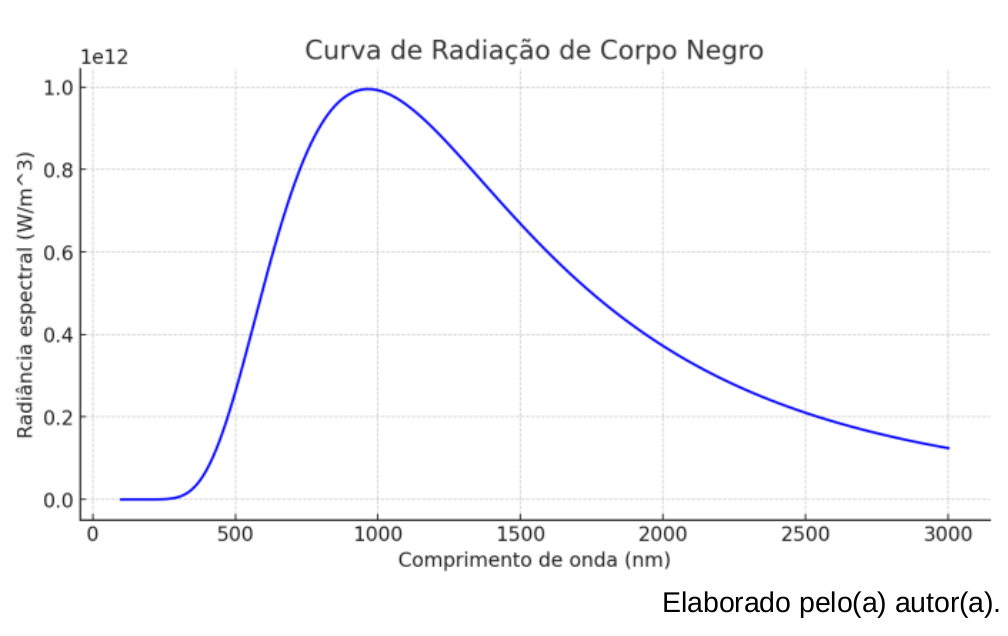
\includegraphics[scale=0.5]{figures/radiacaocorponegro.png}
\end{figure}

O gráfico acima mostra a curva de radiância espectral de um
corpo negro, com o pico da emissão ocorrendo em 966 nm.
Utilizando a Lei de Wien, que relaciona o comprimento de
onda de pico da emissão de um corpo negro com a sua
temperatura, selecione a resposta que mais se aproxima do
resultado calculado para a temperatura desse corpo negro.
(Dados: Constante de deslocamento de Wien $b = 2{,}897 \times 10^{-3}\,\mathrm{m}\,.\mathrm{K}.)$

\begin{itemize}
\item[(A)] 3000 K.
\item[(B)] 3100 K.
\item[(C)] 3300 K.
\item[(D)] 3900 K.
\end{itemize}

\vspace{0.5cm}

\textcolor{red}{\textbf{Solução:}}\\

\section*{Determinação da temperatura de um corpo negro usando a lei de Wien}

A \textbf{lei do deslocamento de Wien} estabelece que:
\[
\lambda_{\text{pico}} \cdot T = b
\]

onde:
\begin{itemize}
    \item \( \lambda_{\text{pico}} \) é o comprimento de onda no qual a radiância espectral é máxima (em metros),
    \item \( T \) é a temperatura absoluta do corpo negro (em kelvins),
    \item \( b = 2,897 \times 10^{-3} \, \mathrm{m\cdot K} \) é a constante de deslocamento de Wien.
\end{itemize}

\section*{Dados do problema:}

O pico da emissão ocorre em:
\[
\lambda_{\text{pico}} = 966 \, \mathrm{nm} = 966 \times 10^{-9} \, \mathrm{m} = 9,66 \times 10^{-7} \, \mathrm{m}.
\]

\section*{Cálculo da temperatura:}

A temperatura é dada por:
\[
T = \frac{b}{\lambda_{\text{pico}}}
\]

Substituindo os valores:
\[
T = \frac{2,897 \times 10^{-3}}{9,66 \times 10^{-7}}.
\]

Efetuando a divisão:
\[
T \approx 2998 \, \mathrm{K}.
\]

\section*{Resposta final:}

\[
\boxed{
T \approx 3000 \, \mathrm{K}
}
\]

Portanto, a temperatura do corpo negro é aproximadamente \( \mathbf{3000\,K} \).

A resposta correta é alternativa \colorbox{green!50}{\textbf{A}}.
\end{flushleft}

\noindent\rule{\linewidth}{0.6pt}\\

\begin{flushleft}
\textbf{\textcolor{blue}{\Large Q53}}\\
\noindent
Uma superfície metálica é exposta a luz de comprimento de onda de 400 nm para induzir o efeito fotoelétrico. A função
trabalho do metal é de 2,0 eV. São dadas a Constante de Planck $h = 6{,}626 \times 10^{-34} J.s$, a velocidade da luz 
$c = 3{,}0 \times 10^8 m/s$ e $e = 1{,}602 \times 10^{-19} J$. Utilizando a equação do efeito fotoelétrico podemos 
determinar a energia cinética máxima dos elétrons ejetados da superfície metálica, que

\begin{itemize}
\item[(A)] 0,95 eV.
\item[(B)] 1,10 eV.
\item[(C)] 1,25 eV.
\item[(D)] 1,50 eV.
\end{itemize}

\vspace{0.5cm}

\textcolor{red}{\textbf{Solução:}}\\

\section*{Efeito Fotoelétrico: Cálculo da energia cinética máxima}

Uma superfície metálica é iluminada com luz de comprimento de onda \( \lambda = 400\,\mathrm{nm} \), e sua função trabalho é:
\[
W_0 = 2{,}0\,\mathrm{eV}.
\]

Queremos calcular a energia cinética máxima \( K_{\text{máx}} \) dos elétrons ejetados.

\section*{Equação do efeito fotoelétrico}

A equação do efeito fotoelétrico é:
\[
E_f = W_0 + K_{\text{máx}},
\]
onde \(E_f\) é a energia do fóton incidente:
\[
E_f = h\nu = \frac{hc}{\lambda}.
\]

\section*{Conversão de unidades}

O comprimento de onda em metros:
\[
\lambda = 400\,\mathrm{nm} = 400 \times 10^{-9}\,\mathrm{m}.
\]

A constante de Planck:
\[
h = 6{,}626 \times 10^{-34}\, \mathrm{J\cdot s}.
\]

Velocidade da luz:
\[
c = 3{,}0 \times 10^{8}\, \mathrm{m/s}.
\]

\section*{Energia do fóton}

Calculamos \(E_f\) em joules:
\[
E_f = \frac{hc}{\lambda} =
\frac{6{,}626 \times 10^{-34} \cdot 3{,}0 \times 10^{8}}{400 \times 10^{-9}}.
\]

Efetuando a conta:
\[
E_f \approx 4{,}97 \times 10^{-19}\, \mathrm{J}.
\]

Convertendo para elétron-volts (\(1\,\mathrm{eV} = 1{,}602 \times 10^{-19}\,\mathrm{J}\)):
\[
E_f = \frac{4{,}97 \times 10^{-19}}{1{,}602 \times 10^{-19}} \approx 3,1\,\mathrm{eV}.
\]

\section*{Energia cinética máxima}

Usamos:
\[
K_{\text{máx}} = E_f - W_0.
\]

Substituindo os valores:
\[
K_{\text{máx}} = 3{,}1\,\mathrm{eV} - 2{,}0\,\mathrm{eV} = 1{,}1\,\mathrm{eV}.
\]

\section*{Resposta final}

\[
\boxed{
K_{\text{máx}} \approx 1{,}1\,\mathrm{eV}
}
\]

A energia cinética máxima dos elétrons ejetados é aproximadamente \(1{,}1\,\mathrm{eV}\).

A resposta correta é alternativa \colorbox{green!50}{\textbf{B}}.
\end{flushleft}

\noindent\rule{\linewidth}{0.6pt}\\

\begin{flushleft}
\textbf{\textcolor{blue}{\Large Q54}}\\
\noindent
No efeito fotoelétrico ocorre a emissão de elétrons de uma
superfície metálica quando radiação incide sobre essa
superfície. A radiação mais eficaz para que o efeito
fotoelétrico ocorra é a

\begin{itemize}
\item[(A)] radiação de raios X.
\item[(B)] radiação infravermelha.
\item[(C)] radiação ultravioleta.
\item[(D)] radiação de micro-ondas.
\end{itemize}

\vspace{0.5cm}

\textcolor{red}{\textbf{Solução:}}\\

\section*{Efeito Fotoelétrico: Resolução e valores típicos da função trabalho}

Quando luz incide sobre a superfície de um metal, elétrons podem ser ejetados se a energia do fóton \( E_f \) for maior ou igual à função trabalho \( W_0 \) do metal:
\[
E_f = W_0 + K_{\text{máx}}
\]

onde:
\begin{itemize}
    \item \( E_f = \frac{hc}{\lambda} \) é a energia do fóton;
    \item \( W_0 \) é a função trabalho do metal;
    \item \( K_{\text{máx}} \) é a energia cinética máxima dos elétrons.
\end{itemize}

\section*{Resolução do problema:}

\textbf{Dados:}
\[
\lambda = 400\,\mathrm{nm}, \quad W_0 = 2{,}0\,\mathrm{eV}, \quad hc = 1240\,\mathrm{eV\cdot nm}.
\]

Energia do fóton:
\[
E_f = \frac{1240}{400} = 3{,}1\,\mathrm{eV}.
\]

Energia cinética máxima:
\[
K_{\text{máx}} = E_f - W_0 = 3{,}1 - 2{,}0 = 1{,}1\,\mathrm{eV}.
\]

\textbf{Resposta:}
\[
\boxed{
K_{\text{máx}} \approx 1{,}1\,\mathrm{eV}
}
\]

\section*{Função trabalho de alguns metais e comprimentos de onda limites:}

A função trabalho \( W_0 \) está relacionada ao comprimento de onda máximo \( \lambda_{\text{lim}} \) para que o efeito fotoelétrico ocorra:
\[
\lambda_{\text{lim}} = \frac{hc}{W_0}
\]

com \( hc = 1240\,\mathrm{eV\cdot nm} \).

\bigskip

\begin{center}
\renewcommand{\arraystretch}{1.3}
\begin{tabular}{|c|c|c|}
\hline
\textbf{Metal} & \textbf{Função trabalho \( W_0~(\mathrm{eV}) \)} & \textbf{\( \lambda_{\text{lim}}~(\mathrm{nm}) \)} \\
\hline
Césio (Cs)     & 1,9 & 653 \\ \hline
Potássio (K)   & 2,3 & 539 \\ \hline
Sódio (Na)     & 2,7 & 459 \\ \hline
Cálcio (Ca)    & 3,2 & 388 \\ \hline
Cobre (Cu)     & 4,7 & 264 \\ \hline
Prata (Ag)     & 4,3 & 288 \\ \hline
Ouro (Au)      & 5,1 & 243 \\ \hline
\hline
\end{tabular}
\end{center}

\section*{Resumo:}
\begin{itemize}
    \item A energia cinética máxima dos elétrons ejetados é a diferença entre a energia do fóton incidente e a função trabalho.
    \item Quanto menor a função trabalho, maior o comprimento de onda limite para o efeito fotoelétrico.
    \item Metais alcalinos (como césio e potássio) são mais fáceis de ionizar.
\end{itemize}

A resposta correta é alternativa \colorbox{green!50}{\textbf{C}}.
\end{flushleft}

\noindent\rule{\linewidth}{0.6pt}\\

\begin{flushleft}
\textbf{\textcolor{blue}{\Large Q55}}\\
\noindent
Um fóton com um comprimento de onda inicial de \(0,10\,\text{nm}\) colide com um elétron inicialmente em repouso.  
Após a colisão, o fóton é espalhado com um ângulo de \(60^\circ\) em relação à sua direção original.  
Sabendo que \(\cos 60^\circ = 0,5\), dada a constante de Compton \(2,43 \times 10^{-12}\,m\) e usando a fórmula do 
efeito Compton para calcular a mudança no comprimento de onda do fóton espalhado, podemos determinar o novo comprimento 
de onda do fóton após o espalhamento, que é de:


\begin{itemize}
\item[(A)] 0{,}102 nm.
\item[(B)] 0{,}222 nm.
\item[(C)] 0{,}220 nm.
\item[(D)] 0{,}232 nm.
\end{itemize}

\vspace{0.5cm}

\textcolor{red}{\textbf{Solução:}}\\

\section*{Efeito Compton: Cálculo do novo comprimento de onda do fóton}

Um fóton com comprimento de onda inicial:
\[
\lambda_0 = 0{,}10\,\mathrm{nm} = 1{,}0 \times 10^{-10}\,\mathrm{m}
\]

é espalhado por um elétron inicialmente em repouso, formando um ângulo de:
\[
\theta = 60^\circ.
\]

Sabemos que:
\[
\cos 60^\circ = 0{,}5
\]

e a \textbf{constante de Compton} do elétron é:
\[
\lambda_C = 2{,}43 \times 10^{-12}\,\mathrm{m}.
\]

\section*{Fórmula do efeito Compton}

A variação no comprimento de onda do fóton é dada por:
\[
\Delta \lambda = \lambda_C (1 - \cos\theta)
\]

Substituindo os valores:
\[
\Delta \lambda =
2{,}43 \times 10^{-12} \cdot (1 - 0{,}5) =
2{,}43 \times 10^{-12} \cdot 0{,}5 =
1{,}215 \times 10^{-12}\,\mathrm{m}.
\]

\section*{Novo comprimento de onda}

O novo comprimento de onda do fóton é:
\[
\lambda = \lambda_0 + \Delta\lambda
\]

Substituindo:
\[
\lambda =
1{,}0 \times 10^{-10} + 1{,}215 \times 10^{-12} =
1{,}01215 \times 10^{-10}\,\mathrm{m}.
\]

Convertendo para nanômetros (\(1\,\mathrm{nm} = 10^{-9}\,\mathrm{m}\)):
\[
\lambda =
0{,}101215\,\mathrm{nm}.
\]

\section*{Resposta final}

\[
\boxed{
\lambda \approx 0{,}1012\,\mathrm{nm}
}
\]

O novo comprimento de onda do fóton espalhado é aproximadamente \(0{,}1012\,\mathrm{nm}\).

A resposta correta é alternativa \colorbox{green!50}{\textbf{A}}.
\end{flushleft}

\noindent\rule{\linewidth}{0.6pt}\\

\begin{flushleft}
\textbf{\textcolor{blue}{\Large Q56}}\\
\noindent
No efeito Compton, um fóton incide sobre um elétron inicialmente em repouso e é espalhado, fazendo com que o elétron recue.  
Quando o ângulo de espalhamento \( \varphi \) varia de \(0^\circ\) a \(90^\circ\), o ângulo de recuo do elétron \( \theta \) 
varia no intervalo:


\begin{itemize}
\item[(A)] $0^{\circ} \leq \theta \leq 180^{\circ}$.
\item[(B)] $0^{\circ} \leq \theta < 90^{\circ}$.
\item[(C)] $0^{\circ} \leq \theta < 120^{\circ}$.
\item[(D)] $90^{\circ} \leq \theta < 120^{\circ}$.
\end{itemize}

\vspace{0.5cm}

\textcolor{red}{\textbf{Solução:}}\\

\section*{Demonstração da relação entre os ângulos no efeito Compton}

No efeito Compton, um fóton incide com momento \( \vec{p}_\gamma \) e energia \( E_\gamma = h\nu \) sobre um elétron em repouso.  
Após a colisão:
\begin{itemize}
    \item o fóton é espalhado com ângulo \( \varphi \) e comprimento de onda aumentado (\( \lambda' \)),
    \item o elétron recua com ângulo \( \theta \) e energia cinética \( K \).
\end{itemize}

\subsection*{Conservação da quantidade de movimento}

No sistema de coordenadas onde o fóton inicial se propaga ao longo do eixo \(x\), temos:
\[
\vec{p}_\gamma = p_\gamma \hat{x}
\]

e após a colisão:
\[
\vec{p}_\gamma' = p_\gamma' \bigl( \cos\varphi\,\hat{x} + \sin\varphi\,\hat{y} \bigr)
\]
\[
\vec{p}_e = p_e \bigl( \cos\theta\,\hat{x} + \sin\theta\,\hat{y} \bigr)
\]

\subsection*{Componentes no eixo \(x\)}

\[
p_\gamma = p_\gamma' \cos\varphi + p_e \cos\theta
\]

\subsection*{Componentes no eixo \(y\)}

\[
0 = p_\gamma' \sin\varphi - p_e \sin\theta
\]

Da segunda equação, obtemos:
\[
p_e \sin\theta = p_\gamma' \sin\varphi
\]

Da primeira equação, isolamos \( p_e \cos\theta \):
\[
p_e \cos\theta = p_\gamma - p_\gamma' \cos\varphi
\]

\subsection*{Tangente do ângulo \( \theta \)}

Dividindo as componentes \(y/x\), temos:
\[
\tan\theta = \frac{p_e \sin\theta}{p_e \cos\theta} =
\frac{p_\gamma' \sin\varphi}{p_\gamma - p_\gamma' \cos\varphi}
\]

\subsection*{Expressando em termos de energias}

Sabemos que \( p_\gamma = \frac{E_\gamma}{c} \) e \( p_\gamma' = \frac{E_\gamma'}{c} \), onde \( E_\gamma' \) é a energia do fóton espalhado:
\[
E_\gamma' = \frac{E_\gamma}{1 + \frac{E_\gamma}{m_e c^2}(1 - \cos\varphi)}
\]

Substituímos \( p_\gamma' \) na equação anterior para obter \( \tan\theta \) em função de \( \varphi \) e \( E_\gamma \).

\section*{Resultado final:}

A relação geral é:
\[
\tan\theta =
\frac{\sin\varphi}{\displaystyle \frac{E_\gamma}{E_\gamma'} - \cos\varphi}
\]

ou ainda, substituindo \( E_\gamma' \):
\[
\tan\theta =
\frac{\sin\varphi}{\displaystyle \left( 1 + \frac{E_\gamma}{m_e c^2}(1 - \cos\varphi) \right) - \cos\varphi}
\]

Essa é a relação entre o ângulo de espalhamento do fóton \( \varphi \) e o ângulo de recuo do elétron \( \theta \) no efeito Compton.

O \(E_\gamma\) é a energia inicial do fóton, e definimos a razão adimensional:

\[
\alpha =
\frac{E_\gamma}{m_e c^2}.
\]

Substituindo \(\alpha\), a expressão fica:

\[
\tan\theta =
\frac{\sin\varphi}{
\big(1 + \alpha(1-\cos\varphi)\big) - \cos\varphi}.
\]

\section*{Limite quando \(\varphi \to 0^\circ\)}

Para \(\varphi \to 0^\circ\), temos:
\[
\sin\varphi \to 0, \quad \cos\varphi \to 1.
\]

No denominador:
\[
\big(1 + \alpha(1-\cos\varphi)\big) - \cos\varphi 
\to (1 + 0) - 1 = 0.
\]

Portanto:
\[
\tan\theta \to 0 \quad \implies \quad \theta \to 0.
\]

\section*{Limite quando \(\varphi = 90^\circ\)}

Para \(\varphi = 90^\circ\), temos:
\[
\sin\varphi = 1, \quad \cos\varphi = 0.
\]

No denominador:
\[
\big(1 + \alpha(1-0)\big) - 0 =
1 + \alpha.
\]

Logo:
\[
\tan\theta =
\frac{1}{1+\alpha}.
\]

Observações:
\begin{itemize}
    \item Para fótons de baixa energia (\(\alpha \ll 1\)): \(1+\alpha \approx1\), então \(\tan\theta\approx1\), ou seja, \(\theta\approx45^\circ\).
    \item Para fótons de alta energia (\(\alpha\gg1\)): \(1+\alpha\) é grande, então \(\tan\theta\approx0\), ou seja, \(\theta\) pequeno.
\end{itemize}

Portanto, mesmo para \(\varphi=90^\circ\), o ângulo \(\theta\) permanece \textbf{menor que \(90^\circ\)}.

\section*{Conclusão}

O ângulo de recuo do elétron \(\theta\) varia no intervalo:
\[
\boxed{0^\circ \leq \theta < 90^\circ}
\]


A resposta correta é alternativa \colorbox{green!50}{\textbf{B}}.
\end{flushleft}

\noindent\rule{\linewidth}{0.6pt}\\

\begin{flushleft}
\textbf{\textcolor{blue}{\Large Q57}}\\
\noindent
Sabendo que a massa do elétron é \( 9,11 \times 10^{-31}\, \mathrm{kg} \), a velocidade da luz é 
\( 3 \times 10^8\, \mathrm{m/s} \) e \( 1\,\mathrm{eV} = 1{,}602 \times 10^{-19}\, \mathrm{J} \), 
a energia total de um elétron movendo-se com uma velocidade de \( \left( \frac{\sqrt{3}}{2} \right) c \) é de:

\begin{itemize}
\item[(A)] $0{,}510$ MeV.
\item[(B)] $0{,}723$ MeV.
\item[(C)] $1{,}024$ MeV.
\item[(D)] $1{,}105$ MeV.
\end{itemize}

\vspace{0.5cm}

\textcolor{red}{\textbf{Solução:}}\\

\section*{Cálculo da energia total relativística do elétron}

\textbf{Dados:}
\begin{itemize}
    \item Massa do elétron: \(m_e = 9{,}11 \times 10^{-31}\, \mathrm{kg}\)
    \item Velocidade da luz: \(c = 3{,}0 \times 10^8\, \mathrm{m/s}\)
    \item \(1\,\mathrm{eV} = 1{,}602 \times 10^{-19}\, \mathrm{J}\)
    \item Velocidade do elétron: \(v = \frac{\sqrt{3}}{2} c\)
\end{itemize}

\subsection*{Fator de Lorentz}

A energia total relativística do elétron é dada por:
\[
E = \gamma m_e c^2
\]

com o fator de Lorentz:
\[
\gamma = \frac{1}{\sqrt{1 - \frac{v^2}{c^2}}}
\]

Sabemos que:
\[
\frac{v}{c} = \frac{\sqrt{3}}{2} \quad \implies \quad \left( \frac{v}{c} \right)^2 = \frac{3}{4}
\]

Portanto:
\[
\gamma = \frac{1}{\sqrt{1 - \frac{3}{4}}} =
\frac{1}{\sqrt{\frac{1}{4}}} =
2
\]

\subsection*{Energia de repouso do elétron}

A energia de repouso do elétron é:
\[
E_0 = m_e c^2
\]

Substituindo os valores:
\[
E_0 =
\left( 9{,}11 \times 10^{-31} \right) \cdot
\left( 3{,}0 \times 10^8 \right)^2 =
9{,}11 \times 10^{-31} \cdot 9{,}0 \times 10^{16} =
8{,}199 \times 10^{-14}\, \mathrm{J}
\]

\subsection*{Energia total do elétron}

\[
E = \gamma E_0 =
2 \cdot 8{,}199 \times 10^{-14} =
1{,}6398 \times 10^{-13}\, \mathrm{J}
\]

\subsection*{Conversão para eV}

Sabemos que \(1\,\mathrm{eV} = 1{,}602 \times 10^{-19}\, \mathrm{J}\), então:
\[
E =
\frac{1{,}6398 \times 10^{-13}}{1{,}602 \times 10^{-19}} \approx
1{,}024 \times 10^6\, \mathrm{eV} =
1{,}024\,\mathrm{MeV}
\]

\subsection*{Resposta final:}

\[
\boxed{
E \approx 1{,}02\, \mathrm{MeV}
}
\]

\textbf{A energia total do elétron em movimento com velocidade \( \frac{\sqrt{3}}{2}c \) é aproximadamente: \(1{,}02\,\mathrm{MeV}\).}

A resposta correta é alternativa \colorbox{green!50}{\textbf{C}}.
\end{flushleft}

\noindent\rule{\linewidth}{0.6pt}\\

\begin{flushleft}
\textbf{\textcolor{blue}{\Large Q58}}\\
\noindent
Uma nave espacial viaja a uma velocidade de \(0{,}85c\) em relação à Terra, sendo \(c = 3 \times 10^8\, \mathrm{m/s}\) 
a velocidade da luz no vácuo. Um relógio a bordo da nave marca 1 hora. Aproximando \( \sqrt{0{,}2775} = 0{,}53 \), 
durante esse tempo a distância percorrida e o tempo decorrido para um observador na Terra são, respectivamente:


\begin{itemize}
\item[(A)] Distância: \(1{,}7 \times 10^9\, km\), Tempo: \(1{,}9\) horas.
\item[(B)] Distância: \(1{,}7 \times 10^9\, km\), Tempo: \(3{,}8\) horas.
\item[(C)] Distância: \(3{,}1 \times 10^8\, km\), Tempo: \(2{,}9\) horas.
\item[(D)] Distância: \(3{,}1 \times 10^8\, km\), Tempo: \(3{,}9\) horas.
\end{itemize}

\vspace{0.5cm}

\textcolor{red}{\textbf{Solução:}}\\

\section*{Problema: nave viajando a \(0{,}85c\)}

Uma nave espacial viaja a uma velocidade \(v = 0{,}85c\), com \(c = 3{,}0 \times 10^8\, \mathrm{m/s}\).  
O relógio a bordo da nave marca um tempo próprio \(t_0 = 1\,\mathrm{h}\).  
Sabendo que \(\sqrt{0{,}2775} = 0{,}53\), queremos calcular:

\begin{itemize}
    \item A distância percorrida para um observador na Terra.
    \item O tempo decorrido para um observador na Terra.
\end{itemize}

\subsection*{Fator de Lorentz}

O tempo medido na Terra é dilatado:
\[
t = \gamma t_0
\]

com:
\[
\gamma = \frac{1}{\sqrt{1-\frac{v^2}{c^2}}}
\]

Calculamos:
\[
\left( \frac{v}{c} \right) = 0{,}85 \quad \implies \quad \left( \frac{v}{c} \right)^2 = 0{,}7225
\]

Logo:
\[
1 - \frac{v^2}{c^2} = 1 - 0{,}7225 = 0{,}2775
\]

Como \(\sqrt{0{,}2775} = 0{,}53\), temos:
\[
\gamma = \frac{1}{0{,}53} \approx 1{,}89
\]

Assim:
\[
t = \gamma t_0 = 1{,}89 \cdot 1 = 1{,}89\,\mathrm{h} \approx 1{,}9\,\mathrm{h}
\]

\subsection*{Distância percorrida na Terra}

Na Terra, a distância percorrida é:
\[
d = v t
\]

com:
\[
v = 0{,}85 \cdot 3{,}0 \times 10^8 = 2{,}55 \times 10^8\, \mathrm{m/s}
\]

Convertendo \(t = 1{,}9\,\mathrm{h}\) para segundos:
\[
t = 1{,}9 \cdot 3600 = 6840\,\mathrm{s}
\]

Então:
\[
d = 2{,}55 \times 10^8 \cdot 6840 \approx 1{,}744 \times 10^{12}\,\mathrm{m} = 1{,}744 \times 10^9\,\mathrm{km} \approx 1{,}7 \times 10^9\,\mathrm{km}
\]

\subsection*{Resposta final:}

\[
\boxed{
\text{Distância: } 1{,}7 \times 10^9\,\mathrm{km} \quad \text{Tempo: } 1{,}9\,\mathrm{h}
}
\]


A resposta correta é alternativa \colorbox{green!50}{\textbf{A}}.
\end{flushleft}

\noindent\rule{\linewidth}{0.6pt}\\


\begin{flushleft}
\textbf{\textcolor{blue}{\Large Q59}}\\
\noindent
Um hospital utiliza o isótopo radioativo Tecnécio-99m (\(^{99m}\mathrm{Tc}\)) para exames de diagnóstico por imagem.  
O Tecnécio-99m tem uma meia-vida de aproximadamente \(6\) horas. Se uma dose inicial de \(120\,\mathrm{mg}\) de Tecnécio-99m é 
administrada a um paciente, quanto tempo será necessário para que a quantidade de isótopo no corpo do paciente caia para \(15\,\mathrm{mg}\)?
(Dados: \(\ln 2 = 0{,}693\) e \(\ln(0{,}125) = -2{,}079\).)

\begin{itemize}
\item[(A)] 10 horas.
\item[(B)] 12 horas.
\item[(C)] 14 horas.
\item[(D)] 18 horas.
\end{itemize}

\vspace{0.5cm}

\textcolor{red}{\textbf{Solução:}}\\

\text{Dados:}

\begin{itemize}
    \item Meia-vida do Tecnécio-99m: \( T_{1/2} = 6 \) horas
    \item Dose inicial: \( N_0 = 120\,\mathrm{mg} \)
    \item Dose final desejada: \( N = 15\,\mathrm{mg} \)
    \item \(\ln 2 = 0{,}693\)
    \item \(\ln(0{,}125) = -2{,}079\)
\end{itemize}

\vspace{0.3cm}

\text{A quantidade de isótopo após um tempo \(t\) é dada por:}

\[
N = N_0 e^{-\lambda t}
\]

\text{onde \(\lambda\) é a constante de decaimento.}

\vspace{0.3cm}

\text{A constante \(\lambda\) está relacionada à meia-vida por:}

\[
T_{1/2} = \frac{\ln 2}{\lambda} \implies \lambda = \frac{\ln 2}{T_{1/2}} = \frac{0{,}693}{6} = 0{,}1155\,\mathrm{h}^{-1}
\]

\vspace{0.3cm}

\text{Queremos o tempo \(t\) para que a quantidade caia para \(15\,\mathrm{mg}\), ou seja:}

\[
\frac{N}{N_0} = e^{-\lambda t} \implies \ln\left(\frac{N}{N_0}\right) = -\lambda t \implies t = -\frac{1}{\lambda} \ln\left(\frac{N}{N_0}\right)
\]

\vspace{0.3cm}

\text{Calculando:}

\[
\frac{N}{N_0} = \frac{15}{120} = 0{,}125
\]

\[
t = -\frac{1}{0{,}1155} \ln(0{,}125) = -\frac{1}{0{,}1155} \times (-2{,}079) = \frac{2{,}079}{0{,}1155} \approx 18 \text{ horas}
\]

\vspace{0.3cm}

\boxed{
\text{Resposta: } t \approx 18 \text{ horas}}

A resposta correta é alternativa \colorbox{green!50}{\textbf{D}}.
\end{flushleft}

\noindent\rule{\linewidth}{0.6pt}\\

\begin{flushleft}
\textbf{\textcolor{blue}{\Large Q60}}\\
\noindent
Durante uma escavação arqueológica, um arqueólogo encontra restos de uma antiga fogueira contendo pedaços de madeira.  
A atividade do carbono-14 na amostra de madeira é medida e encontrada como sendo \(12{,}5\%\) da atividade do carbono-14 em organismos vivos.  
Sabendo que a meia-vida do carbono-14 é de aproximadamente \(5730\) anos, a idade da amostra de madeira pode ser determinada e vale:  
(Dados: \(\ln 2 = 0{,}693\) e \(\ln(0{,}125) = -2{,}079\).)

\begin{itemize}
\item[(A)] 5.730 anos.
\item[(B)] 8.585 anos.
\item[(C)] 11.460 anos.
\item[(D)] 17.190 anos.
\end{itemize}

\vspace{0.5cm}

\textcolor{red}{\textbf{Solução:}}\\

\text{Dados:}

\begin{itemize}
    \item Fração da atividade atual em relação à original: \(\frac{N}{N_0} = 12{,}5\% = 0{,}125\)
    \item Meia-vida do carbono-14: \(T_{1/2} = 5730 \text{ anos}\)
    \item \(\ln 2 = 0{,}693\)
    \item \(\ln(0{,}125) = -2{,}079\)
\end{itemize}

\vspace{0.3cm}

\text{A atividade após um tempo \(t\) é dada por:}

\[
N = N_0 e^{-\lambda t}
\]

\text{onde \(\lambda\) é a constante de decaimento.}

\vspace{0.3cm}

\text{Calculando \(\lambda\):}

\[
\lambda = \frac{\ln 2}{T_{1/2}} = \frac{0{,}693}{5730} \approx 1{,}21 \times 10^{-4}\, \text{ano}^{-1}
\]

\vspace{0.3cm}

\text{Determinando o tempo \(t\):}

\[
\frac{N}{N_0} = e^{-\lambda t} \implies \ln\left(\frac{N}{N_0}\right) = -\lambda t \implies t = -\frac{1}{\lambda} \ln\left(\frac{N}{N_0}\right)
\]

\vspace{0.3cm}

\text{Substituindo os valores:}

\[
t = -\frac{1}{1{,}21 \times 10^{-4}} \times \ln(0{,}125) = \frac{2{,}079}{1{,}21 \times 10^{-4}} \approx 17\,190 \text{ anos}
\]

\vspace{0.3cm}

\boxed{
\text{Resposta: } t \approx 17\,190 \text{ anos}
}

A resposta correta é alternativa \colorbox{green!50}{\textbf{D}}.
\end{flushleft}

\noindent\rule{\linewidth}{0.6pt}\\


%\begin{flushleft}
%\textbf{\textcolor{blue}{\Large Q52}}\\
%\noindent
%
%\begin{itemize}
%\item[(A)] 
%\item[(B)] 
%\item[(C)] 
%\item[(D)] 
%\end{itemize}
%
%\vspace{0.5cm}
%
%\textcolor{red}{\textbf{Solução:}}\\
%
%A resposta correta é alternativa \colorbox{green!50}{\textbf{...}}.
%\end{flushleft}
%
%\noindent\rule{\linewidth}{0.6pt}\\


%%%%%%%% Bibliography 
% Os comandos para incluir as referências bibliográficas
%\printingbibliography

\end{document}
